\hypertarget{fig:target:main-map}{}
\begin{figure}[htb]
  \centering
  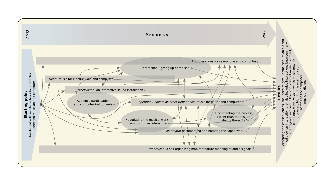
\includegraphics[width=\textwidth]{img/map8-noheader}
  \caption{A timeline with the different sub-projects and themes with their interrelations.}
  \label{fig:main-map}
\end{figure}

% \section{Project background}
% \label{sec:research-question}

\hypertarget{sec:target:introduction-1}{I do not believe} that art is created in solitary confinement but is nurtured in social, human and cultural interaction. Whether my background as a jazz musician and improviser is the explanation for, or a consequence of, this conception holds no real significance for the reading of this book but there is an interesting connection between the sensibility required by an improviser\footnote{Here, I mean the kind of sensibility that George Lewis would refer to as \emph{afrological}: improvisation, in which the personal narrative, manifested partly through the ``personal sound'', is of importance but in which the ``focus of musical discourse suddenly shifts from the individual, autonomous creator to the collective - the individual as a part of global humanity''. \cite[See][110]{lewis-1}} and the sensibility required in any human interaction. 

The primary focus of my PhD project is the interaction between \useGlosentry{glos:musician}{musician} and computer within the context of what is often referred to as \emph{Interactive Music}.
\footcite[See][]{wiki_interactive,Garnett,rowe,winkler01,rowe01} Though this is a commonly used term its meaning is blurred by the magnitude of the concepts that it covers and, in order to unwrap the idea of \index{interaction!musical}musical interaction with a computer, this project also includes other forms of interaction in different contexts and between other kinds of agents as well as different readings of the idea of interaction. These investigations are conducted in the form of reflection on both my artistic and theoretical work. As will be seen, the consequences of the experiences gained from my practice as an improviser and composer may in the end change the way an interactive system, in which a computer is one of the agents, is designed, approached and used. Hence, the study of \useGlosentry{glos:musician}{musician}-musician interaction within this project is not a goal in itself but rather a way to approach the complex field of musician-\index{interaction!computer}computer interaction, which is the type of interaction implied by \emph{Interactive Music}. Similarly, the study of \index{interaction!human-computer}\index{HCI}human-computer interaction is not an end in itself but a way to further understanding of musician-\index{interaction!computer}computer interaction.

%Although human-computer interaction is a very active field of research, its results are not necessarily applicable to the field of art practice. According to interaction researcher Kari \citeauthor{kuutti96} not even software designers are making use of advances in HCI research: ``There is a well-known gap between research results and practical design''.\footcite[18]{kuutti96} \citeauthor{kuutti96} is primarily looking at the interdisciplinary research done in HCI and cognitive psychology and concludes that ``some of the most remarkable new interfaces have been developed with almost no help from research into cognitive psychology''\footcite[18]{kuutti96} If the primary targets for HCI research---interface designers and software developers---are not finding use for it, what is in it for the arts?\footnote{I should remark that a lot has happened in the ten years that has passed since \citeauthor{kuutti96} wrote this article and the surveys and references quoted are almost 20 years old.} The question of the relation between human-computer interaction and the field of art, that is, the question regarding the possibility for a mutual exchange and benefit, will be discussed in more detail in \hyperlink{par:inter-defin:3}{section \ref*{sec:inter-defin}}. Though there are obvious similarities---both are concerned with humans interacting with computers---there are equally obvious dissimilarities.

%This is obviously not to say that HCI research is useless---on the contrary---it is a very important research field with an ever increasing number of applications. But, what is HCI? What does it mean to interact with a computer?

\section{Personal background}
\label{sec:personal-background}

\begin{wrapfigure}{l}{0.15\linewidth}
  \centering
  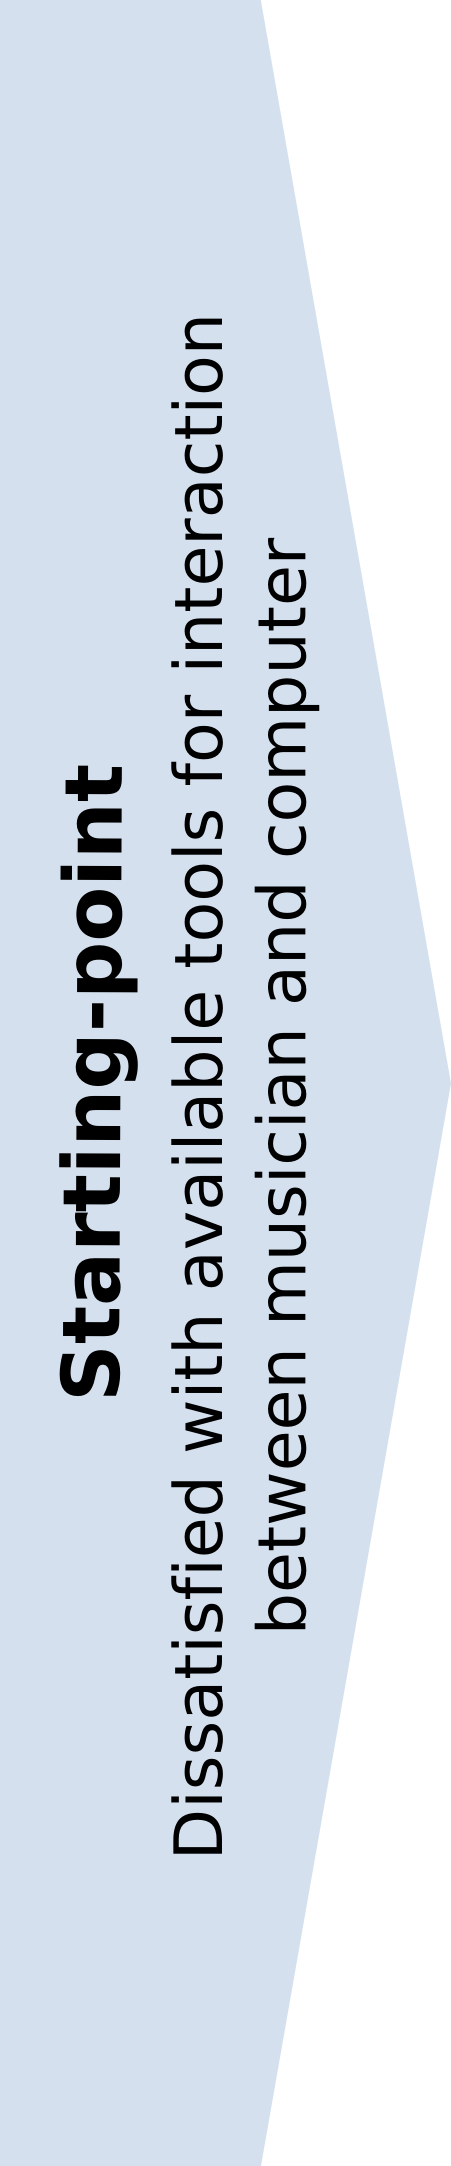
\includegraphics[width=0.5\linewidth]{img/map9-starting-point}
  \label{fig:starting-point}
\end{wrapfigure}

I have two principal areas of interest in my musical practice: improvisation and computers.
\noindent (\emph{i}) As a performer I look at different ways to explore improvisation: idiomatic (primarily jazz) as well as non-idiomatic,\footcite[The terms, `idiomatic' and `non-idiomatic' are borrowed from Derek Bailey. See][]{bailey92} pre-structured and without preparation (as little as is possible), on acoustic instruments and on electronic and home made instruments (mostly \index{software}software instruments on laptop). Even when working with composition in a relatively traditional manner (i.e. using musical notation), I am always looking for ways to allow improvisation to form an integral part of the process. 
At the risk of provoking the controversy about the difference between improvisation and composition,
\footnote{Whether they are part of the same process or different modalities all together depends on whom you ask. Bruno \citeauthor{nettl74} dismantles the composition-improvisation dichotomy replacing it with the idea of points along a continuum. \parencite{nettl74} Towards the end of his influential book on improvisation Derek \citeauthor{bailey92} quotes a discussion in which it was established that ``composition, should there be such a thing, is no different from composition''. \parencite[140]{bailey92} Finally, Bruce Ellis Benson describes improvisation as a property of all musical practices, even composition. \parencite{benson03}} 
%\footcites(Whether they are part of the same process or different modalities all together depends on whom you ask.)()[Bruno Nettl dismantles the composition-improvisation dichotomy replacing it with the idea of points along a continuum.][]{nettl74}[Towards the end of his influential book on improvisation Derek Bailey quotes a discussion in which it was established that ``composition, should there be such a thing, is no different from composition''.][140]{bailey92}[Finally, Bruce Ellis Benson describes improvisation as a property of all musical practices, even composition.][]{benson03}
I must state that in my experience improvisation precedes composition. Composition appears to me to be a more specialised subclass of the practice of improvisation.\footfullcite[These ideas seem to be getting some support from the aforementioned][]{benson03} This relation is also noticeable with regard to \index{interaction!computer}computer interaction, as the strategies I have developed for dealing with the computer's shortcomings\footnote{The computer's shortcomings are dealt with in the chapter on interaction.} while composing do not usually apply to the case of performing, and certainly not to improvising with the computer. Should interaction in the real-time context of improvisation develop and allow for more enunciated dynamics, this would unequivocally inform---and render different---non real-time work such as composing.

\noindent (\emph{ii}) We are constantly surrounded by technology, technology to help us communicate, to travel, to pay our bills, to listen to music, to entertain us, to create excitement in our mundane lives, etc. For the most part, most users are blissfully unaware of what is going on inside the machines that produce the tools we use (the machine itself is usually much more than the tool). There is no way to comprehend it experientially---it is an abstract machine (though not so much in the Deleuzian sense). If a hammer breaks we may reconstruct it on the basis of our experiences of using it but if a computer program breaks the knowledge we have gained from using it is not necessarily useful when, and if, we attempt to mend it. This phenomenon is not (only) tied to the complexity of the machine but is a result of the type of processes the machine initiates and the abstract generality in the technology that implements the tool.\footnote{The abstract Turing machine, the Mother of all computers, is generally thought to be able to solve all logical problems.} I have worked with the computer one way or another in almost all of my artistic work since 1994 and I am still as fascinated by it as I am by the piano or the saxophone. Whereas the piano and the saxophone are already `owned' by music, however, the computer is not. It is subject to constant change and, even though the computer is obviously already an integral part of our culture and a part of our artistic explorations, the speed with which new and faster technology and new technological tools are produced constitutes an unprecedented challenge to anyone interested in incorporating and understanding computers in the frame of a culture that normally proceeds at an entirely different pace. For exactly these reasons, however, I feel a growing responsibility also to explore the computer for artistic purposes---if only to counterbalance the otherwise purely economical considerations surrounding the development and implementation of new computer-based technology. 

My interest in integrating and interacting with electronically produced sounds began in the late 1980s when listening to saxophonists such as Gary Thomas\footcite{thomas88} and Greg Osby
\footcite{dejohnette88} using the IVL Pitchrider\footnote{The IVL Pitchrider is now out of production. At its time it was a state of the art pitch-to-MIDI converter. It took an audio signal from a microphone and sent out a \useGlosentry{glos:MIDI}{MIDI} signal that could be used to control a synthesiser.}, and Frank Zappa playing the Synclavier.\footcite{zappa86,wiki_synclavier} Pat Metheny's use of guitar synthesiser and sampler on the \emph{Song X} record with Ornette Coleman was a thrilling sonic illustration of what could be done relying on what today we would call relatively simple technology.\footcite{metheny86} Later, hearing George Lewis's \emph{Voyager}\footcite{lewis92} I realised the possibilities for something else than the one-to-one mapping between the instrument and the electronics used in the examples above,\footnote{To be honest, it was only when listening to the track \emph{Traf} on Gary Thomas's \emph{Code Violations} that I started thinking about different mapping schemes: ``I assigned a different harmony note to each note I play on the saxophone; I set it up the way I prefer to hear notes run together''. In the same text Thomas makes another interesting remark that had a big impact on me: ``You can take the limitations of tracking technology and turn them into advantages: if you bend a note on the sax, the synth note doesn't bend, so you get some dissonances''. The idea of using the limitations of technology to one's advantage is a way of soft-circuit-bending; using technology in ways and with methods they were originally not intended for. \cite[See cover notes in][\textparagraph 7]{thomas88}} \hypertarget{sec:target:personal-background-1}{described by} \citeauthor{lewis00} ``as multiple parallel streams of music generation, emanating from both the computers and the humans---a non-hierarchical, improvisational, subject-subject model of discourse, rather than a stimulus/response setup''.\footcite[34]{lewis00}

In the early 1990s I was not attached to any academic music institution and I had no computer science training or knowledge. What started at this time was a long process of \emph{reverse-engineering} the sounds I had heard and the processes I was interested in, in the total absence of a terminology or even a language in which to express what I wanted to achieve. The only method available to me was trial and error. In a sense, this book, along with the website\footnote{See \url{http://www.henrikfrisk.com/improvisation.}} is the collection of information, reflection, and documentation that I would have liked to have had access to while taking my first steps in \emph{Interactive Music}. In hindsight I can see that a lot of material, experience and expertise existed but my lack of knowledge and terminology, in combination with my personal and artistic preconditions, made it necessary for me to begin by finding out by myself.

Ten years later I had acquired the knowledge and the expertise to do many of the things I had targeted. Although, however, I was working actively as an improviser and composer with interactive music in different contexts, and though I was able to stage performances with a comparatively high degree of real time interaction between \useGlosentry{glos:musician}{musician}(s) and computer(s), I was not convinced by the \emph{interactive} aspect of the music. In one sense the music was interactive; I used little or no pre-prepared material and many aspects of the shaping of the computer part were governed by performance time parameters, but in another, perhaps more musical, sense it was not interactive at all. At the time, my identification of the source of dissatisfaction was the fact that the information transmitted from musician to machine, once it arrived at the destination in a machine readable format, was no longer of a kind relevant to the music. The information may still have been valid at the source, but when the representation of it was used in the machine to produce sonic material, material that would appear for the musician as a result of the input, the perceptual connection between cause and effect had been lost and with it, I felt, some of the motivation for working with interactive music. One may object to the conclusion that lack of musical relevance of the \emph{signal} at the destination is a problem, arguing instead that the problem is related to a dysfunctional \emph{use} of that signal at the destination. At the time, however, I was convinced that no matter how sophisticated the mapping between input and output would get, or how cleverly the input signal was used, if the extracted information was not meaningful in relation to the way the music was constructed, the interaction as \emph{interaction} would fail (which is not to say that the music would necessarily fail). 

\begin{figure}[ht]
  \centering
  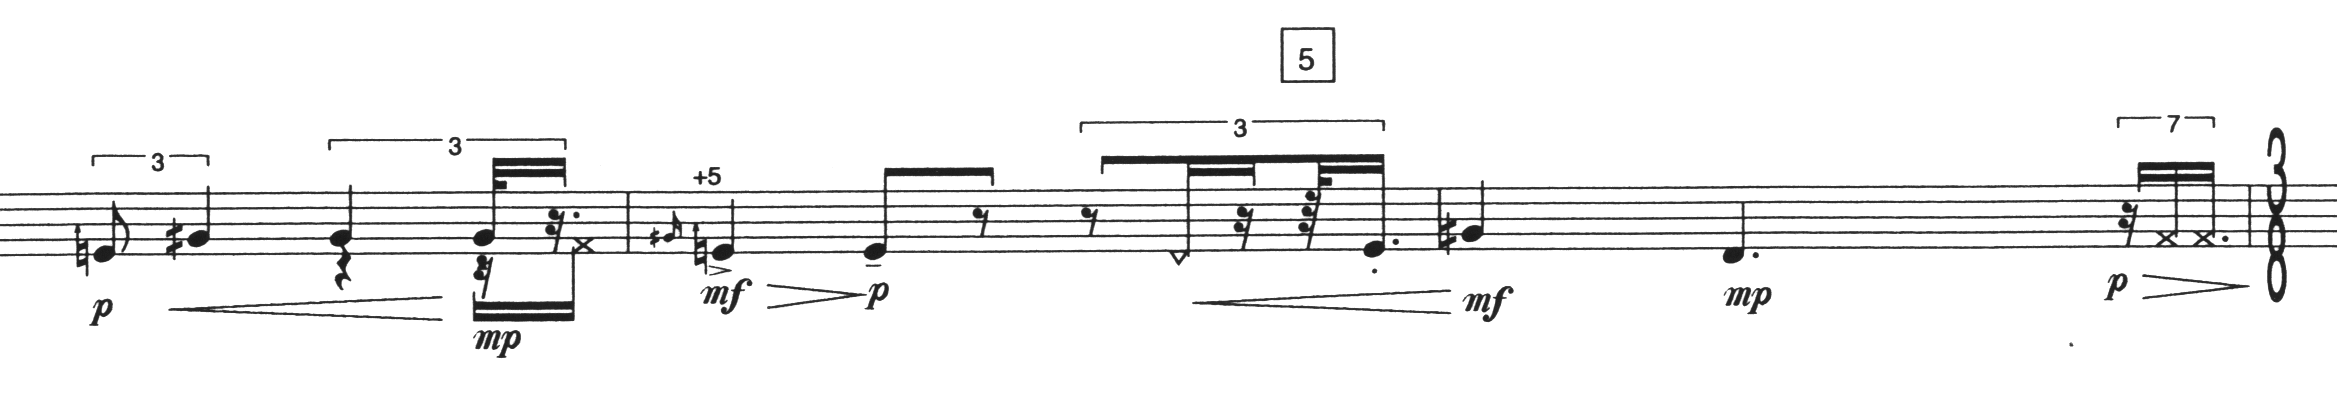
\includegraphics[width=\textwidth]{img/goda-onda}
  \caption[Score excerpt from \citetitle{goda-onda}.]{Score excerpt from the piece \citetitle{goda-onda} by the author. Published by dinergy music pub. \& Svensk Musik}
  \label{fig:goda-onda}
\end{figure}

\hypertarget{sec:target:personal-background-4}{The score excerpt} in Figure \ref{fig:goda-onda} shows bar 3--5 of the flute part of the piece \citetitle{goda-onda} for flute and computer,\footcite[][]{goda-onda} composed 1998/99, and may be used to illustrate one aspect of the problem described above. The piece uses \useGlosentry{glos:pitch-track}{pitch-tracking}\footcite[The pitch-tracking is achieved with the \emph{fiddle\~} object in \index{Max/MSP}Max/MSP. See][]{puckette98} and \index{score following}score-following techniques\footcite[For an overview of \index{score following}score-following techniques, see][chap. 3.2]{rowe} to synchronise the computer with the performer. Overall, in \citetitle{goda-onda}, the \useGlosentry{glos:score_follow}{score-following} works well and is relatively predictable and because the piece is essentially modal, largely owing to the way the modes are composed, the extensive use of micro-tonal variations (e.g. the recurring G quarter tone sharp in the excerpt) does not present a problem. Instead, the issue is the discrepancy of the role pitch has in the structure of the piece on the one hand and in the computer system on the other. Despite the modal nature of the piece, the overriding principle in \citetitle{goda-onda} is not pitch, but rather the way pitched content is combined with non-pitched content, or `regular' flute-sounding notes with ``non-regular'', but what is communicated to the computer is merely the former half of that relation (which in this case is less than half of the information). For example, in the second bar of the note example, the last note, an E (to be played $5/100$ of a tone sharp) is preceded by a D played as a flute pizzicato. Compositionally the `meaning' of the E lies in its relation to the preceding pizzicato tone D and the `meaning' of the D is much more closely related to its timbre than its pitch (which may or may not be a D). None of this information, however, is made accessible to the computer, which is merely receiving information about when a tone is played and what its pitch is.\footnote{In this particular example it may be argued that, if the \index{score following}score-following is functional, information \emph{about} a note (timbre, loudness, articulation, etc.) could be derived from the score rather than the performance. So long as the performance is synchronised with the score, all the information about a given note is (in some cases thought to be) part of the score. \citetitle{goda-onda}, however, contains substantial sections of improvised material where this meta-information is not available prior to performance time. In other words, even if a score-centric (as opposed to performance centred) view is desirable---which it is not to me---it would not work in this composition.} \hypertarget{sec:target:personal-background-2}{Here I located} the source of my frustration: in the computer-performer communication I was limited to one kind of information and that type was not really relevant to the processes I wanted to perform (musically and technically). I saw the solution to this, and other similar problems, in the concept of tracking the timbre, or the relative change of timbre in addition to tracking the pitch.

%; to extract information from the performance of a kind less specialized than pitch only.

If what is described above was the point of departure for this project, although I now more or less have the tools that constitute the first step towards allowing timbre tracking, I have also learned that the problem as described with regard to \citetitle{goda-onda} was badly stated in the sense that it saw the problem, as well as its solution, in far too narrow a way: as a computational task that `only' needed its algorithm. During the course of the project the view on interaction has been broadened to include aspects of interaction that are external to the field of \index{interaction!human-computer}\index{HCI}human-computer interaction. The two main reasons for this may be very briefly summarised as:
(\textit{i}) first of all, interactive music is obviously contingent on kinds of interaction that are not related to the computer. Hence, what is perceived as a dysfunction pertaining to the interactive computer system may under certain conditions be resolved by compensating for it somewhere else, i.e. not necessarily in the computer system itself.
(\textit{ii}) \hypertarget{sec:target:personal-background-3}{second}, regardless of the kind of interaction at work, the attitude towards it and the expectations from it are attributes that consciously or unconsciously shape the design of an interactive system. It is clear that if I expect to be able to \emph{control} an interactive computer (music) system and I fail to do so, I am likely to deem the interactive experience unsatisfactory. From an artistic point of view, however, I will also need to ask myself if expectation of \emph{control} is at all desirable.
In other words, the project started from a relatively narrow view on interaction only to gradually expand it, but without losing the original ambitions, though these would gradually also appear in a new light. The ways in which it expanded, as well as the reasons for the expansion, will be the subject of the following chapters.

\section{The field of research}
\label{sec:summary}

The current PhD project marks an important step in the work in progress for which the goal may be summarised as: to be able to interact dynamically with computers in performances of improvised as well as pre-composed music. `Dynamically' should be understood as non-static in the moment of performance, i.e. \index{real-time}\index{time!real-time}real-time dynamic, but also dynamic with regard to context in non \index{real-time}\index{time!real-time}real-time, as a multiplicity of possibilities: to resist the notion of \emph{the} solution, to defy the \emph{work}, and constantly to re-evaluate and transform according to the changing needs: to opt for the \emph{work-in-movement}. The latter understanding of `dynamic' is furthermore the origin of the concept of re-evaluation of `the \index{Self}Self' that has become central to this project: When 
%the particular solution is dissolved and 
others are allowed entry into the constructive and defining phases of a musical work (which is the consequence of the decomposition of \emph{the work} and the beginning of the \emph{work-in-movement}), the \index{Self}Self of musical production is likewise to be questioned. The significance of these issues was not originally part of the project but was revealed to me while I was working on the \hyperref[sec:ethersound]{interactive sound installation \emph{etherSound}}. As a sound installation it dismantles the relationships between composer, performer and listener. (In relation to \emph{etherSound}, am I the composer, the performer or the listener? Attempting to define one's role, however, is the sign of a relentless articulation of the \index{Self}Self.) Out of these contemplations, in combination with the experiences of audience interaction and participation also gained from \emph{etherSound}, came the notion of \emph{\index{interaction!as difference}\index{interaction-as-difference}interaction-as-difference} as opposed to the common mode of \index{interaction!human-computer}\index{HCI}human-computer interaction, defined here as \emph{\index{interaction!as control}\index{interaction-as-control}interaction-as-control}. 
%In other words, how may the concept `giving up the self' as the first step of human-human interaction on equal terms, and as a possibility for rethinking my musical practice, also be applied to human-computer interaction, in the context of production of musical content?

In this project the (artistic) practice is, in a sense, both the object and the method. The sub-projects contained within the frame of this thesis, some of them still works-in-progress, are used to make inquiries into the larger question of the significance of interaction in the context of artistic practice involving computers. As mentioned above, they are manifestations of different modes of interaction and as such they form the basis for reflections on the subject. Hence, though there are a number of aspects on interaction in relation to computers, musical practice, improvisation and many other topics that could have been followed up, the artistic work has been the proxy that has helped to demarcate and narrow the field of questioning. I should however mention, albeit briefly, one currently influential field that is \emph{not} actively discussed in the present work, but which is very closely related to it. The field of gestural control of music,\footcite[For an overview, see][]{wanderley00} has attracted a great deal of interest within \index{digital}digital media in general and \index{electro-acoustic music}electro-acoustic music in particular in the last decade and includes concepts such as embodiment, immersion and body-sound interaction.\footcites(In the early and mid-1990s \index{virtual}Virtual Reality technology, also in artistic practice, was a source of inspiration for thinking about the role and function of the body in human-technology interaction as well as concepts such as immersion.)()[See][]{moser96}[see also][]{wood98} With no intention of presenting a complete list, I could mention related projects---projects that also share a strong connection to artistic practice as well as to improvisation and/or technology---such as those by pianist and improviser Vijay \citeauthor{iyer08}\footcites[See the PhD thesis][]{iyer98}[See also][]{iyer08} and the saxophonist David \citeauthor{borgo05}.\footcite[Using British saxophonist Evan Parker as a point of demarcation the embodied mind is explored in][chap. 3]{borgo05} They are both examples of improvisers/researchers with a great interest in the study of music and improvisation as an embodied activity. In addition, Norwegian ``music researcher and research musician''\footcite{jensenius08:bio} Alexander \citeauthor{jensenius08}'s recent PhD thesis is a project intimately tied to the author's artistic practice, similarly focused on embodied music cognition and on gesture control of electronic musical instruments.\footcite[See][]{jensenius08}

% In Section \ref{sec:interaction} I will discuss \emph{Interaction} in
% general and then, in Section \ref{sec:interactive-music} I will look
% at that which is commonly referred to as \emph{Interactive Music}.
% That being the meta-level of interaction, I will then proceed to
% discuss the micro-level, the code, or the language and the processes
% of signification---and its nature and quality---and if that may or should
% be considered in interactive music.

%Though this thesis certainly marks the end of one phase, it most certainly, for me personally, also marks the beginning of another.

\newpage
\section{Sub-projects---overview}
\label{sec:overview}

\begin{figure}[!ht]
  \centering
  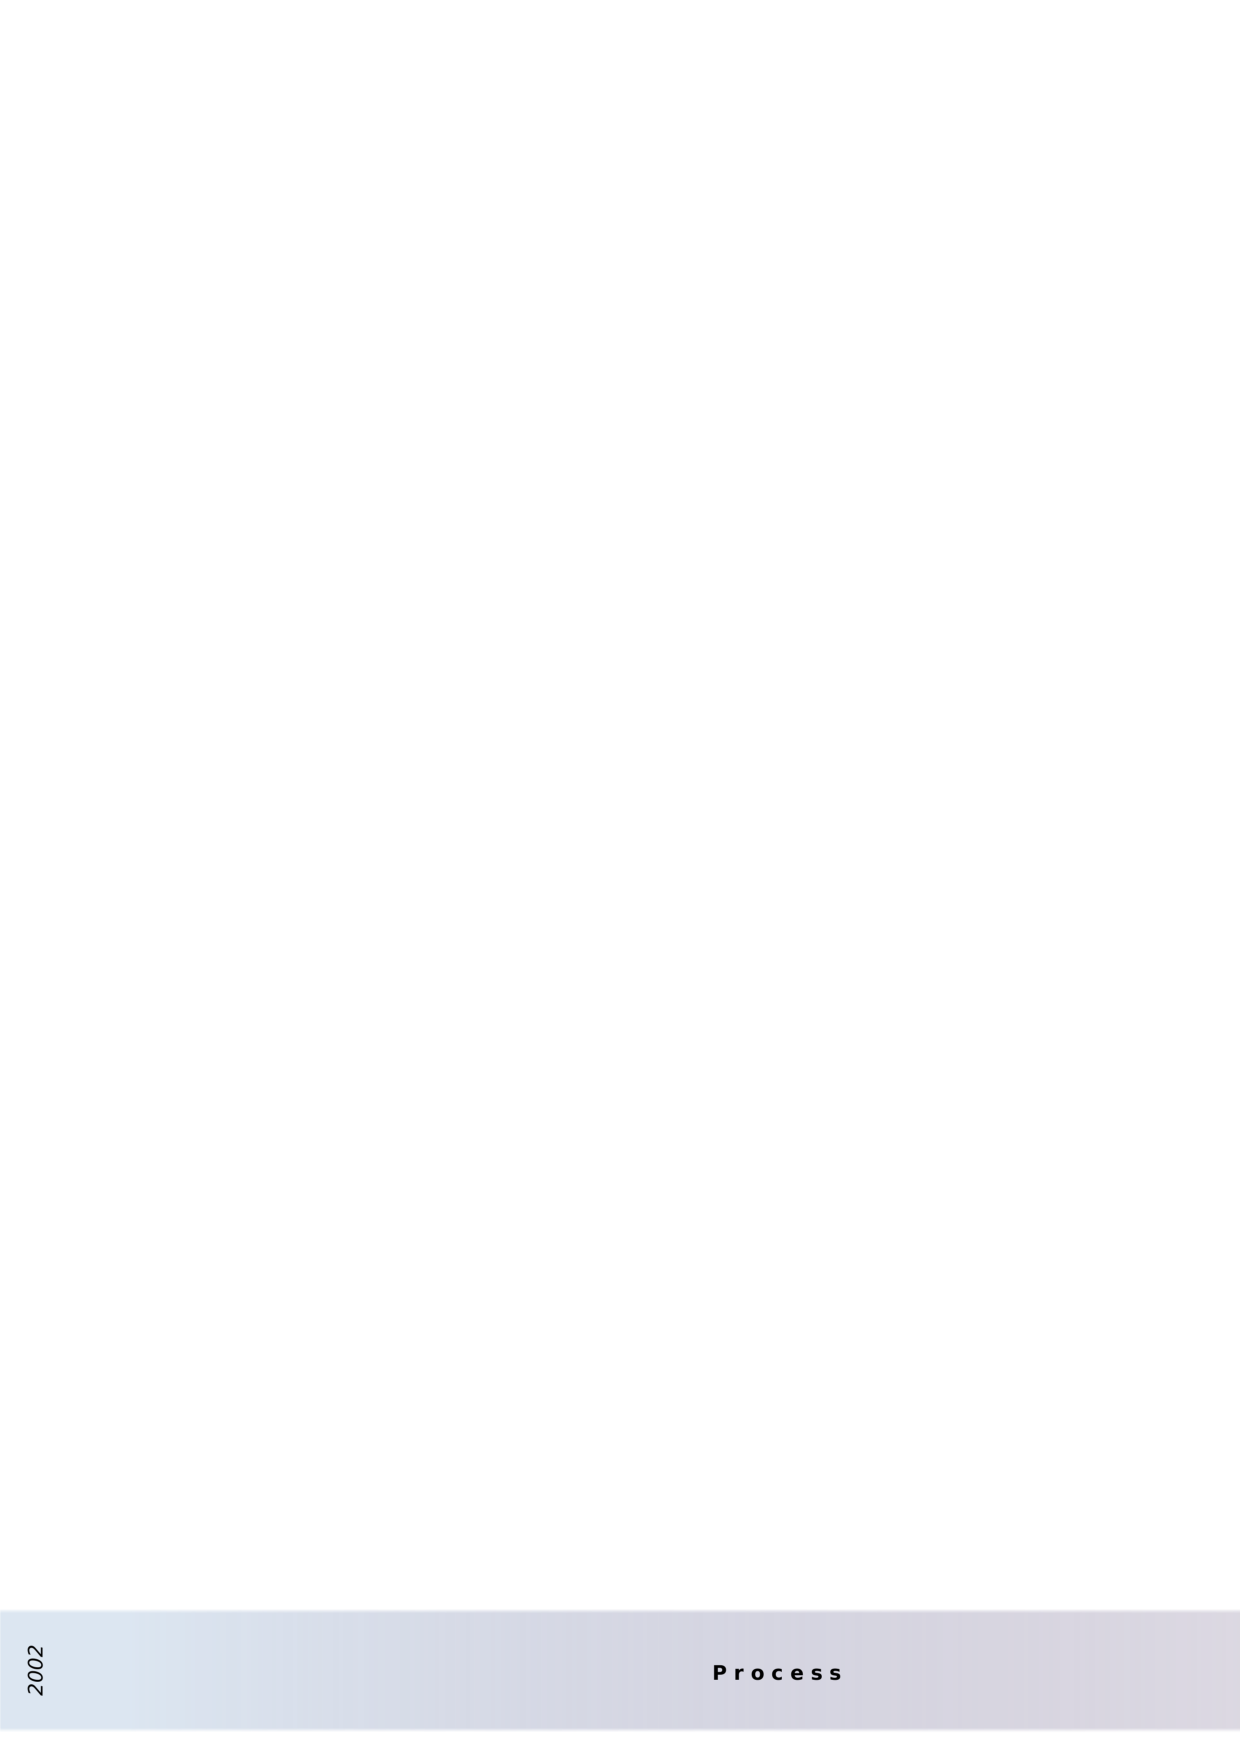
\includegraphics[width=\textwidth]{img/process}
  \caption{Process arrow of project map (See Figure \ref{fig:main-map})}
\end{figure}

This section is intended to function as an annotated table of contents for the reader to get an overview of the project but also to allow for reference look-up of particular components. Although I prefer to see all aspects of this project as a distribution of interrelated parts that overlap with each other, all belonging to my artistic practice, in order to unwrap and make accessible the different facets of import to the thesis, a dissection, so to speak, is necessary. Graphically displayed in \hyperlink{fig:target:main-map}{Figure \ref*{fig:main-map}}, the different enclosures, or sub-projects, are briefly introduced below, but the enclosures are also carriers of artistic experience and have in themselves something to say about the subject matter. The different modes of interaction represented in these artistic projects are not only relating to musician-\index{interaction!computer}computer interaction but also in high degree to musician-musician interaction: interaction taking place in the stages of preparation and development of the projects as well as in the processes of performance, execution and evaluation. Below, the projects appear roughly in the order in which they were initiated in time, but it should be noted that they also extend over time. For example, though \emph{timbreMap} was the first sub-project started, it is also the one that has been active the longest. Although it would be possible to categorise the different sub-projects into `music', `text' and \index{software}`software', in the presentation below I have not done so because I believe it would give a wrong picture of the types of works included here. By resisting this categorisation I hope also to resist the corresponding division of sub-projects into `artistic', `reflective' and `scientific' solely on the basis of their \emph{form}. It is not that I think my music is scientific or my programming is reflective but nor do I think my texts are \emph{only} reflective. For instance, the computer \index{software}software which is part of this project is not merely a ``tool'' to allow for ``testing'' or ``verifying''. I regard it as part of the artistic practice that lies at the very foundation of this project, i.e. as implementations of ideas. They are also beginnings in themselves, however, in that they may, albeit in a limited sense, allow for a different usage of computers in the context of interactive music.

The purpose here is not to draw conclusions that may be \emph{generalised} but rather to test assumptions within the framework of my own artistic production. The \index{software}software, released under the \citetitle{GNUGPL},\footcite{GNUGPL} as well as the music,\footnote{I am currently investigating the consequences of releasing all, or much of my music under the \citetitle{CCLIC}. See \cite{CCLIC}.} may very well be used in other contexts, by other artists for completely different purposes, or to elaborate on the ideas presented in this book. Though programming as an activity is often seen as something done by predominantly asocial men, in isolation, I argue that programming is interaction. It is interaction in order to make the computer interactive, interaction in the language of the computer, but these projects, notably libIntegra, are also in themselves results of higher-level interactions as in group collaboration.\footnote{I would go so far as to say that, based on my own experience, the interaction between myself and Jamie Bullock (the main \index{software}software developer and administrator of the project) was a critical aspect of the development. As the project involved many low level decisions that could potentially be highly significant at a much later stage, there were at times very intensive communication and negotiation between us that in most cases led to new ideas and input in the project. In that sense the interaction was more important than the development.} Many open source \index{software}software development projects interact widely with their users, other developers and other projects.

\hypertarget{sec:target:overview-1}{The computer}, as a physical object (as opposed to the abstract \emph{idea} of the computer), is often intimately coupled with the \index{software}software it hosts, to the degree that operations that are a result of \index{software}software processes are attributed to the computer as object rather than the actual program in question. Furthermore, it is imaginable that, in some cases, these operations should more correctly be associated with the programmer rather than the program. For example, when playing chess against a computer chess program, one has the sensation that the game is played against the \emph{computer}, when in fact the game is played against a dislocated chess game \emph{programmer}.\footcites[See J. Gilmore as quoted in][]{arendt77}[See also][]{baudrillard02:blue} \hyperlink{sec:target:human-comp-inter:par3}{In Section \ref*{sec:human-comp-inter}} the computer operating system is discussed in similar fashion as a sign referring back to the producer of the system. If we can talk about signification in this context the \index{software}software is the sign that holds a causal relation to output of the program, which in turn signifies the origin of the program: the programmer(s) or the context s/he or they belong(s) to. Now, this is not a general clause. To delineate \index{software}software and talk about it as a symbol somewhat independent of its host in this manner is obviously not always possible: compilers and embedded systems are only two examples. In my own practice, however, the idea that programming is a means of positing some part of myself within the \index{software}software, not unlike how writing a musical score is a way to communicate oneself, has become an important aspect. Under certain conditions, the computer, when running \index{software}software I have contributed to, may then be seen to function as a mediator of myself, again similarly to the way a score is a mediator of its composer. The computer acts as a host for a detached \index{Self}self, as an `instantiator' of my imprint, the code, with which I can interact. Contrary to the immediate appearance of ego-centric narcissism in this description---coding the \index{Self}Self to play the \index{Self}Self to interact with the \index{Self}Self---for me, the \index{Self}Self is instead distorted. (Under certain conditions the result could equally well turn out to manifest narcissism.) In the superimposition of different kinds of logic, of \index{Self}Self as sign and \index{Self}Self as \index{Self}Self, and different kinds of time, that of real time and that of detached time, a possibility for losing the \index{Self}Self eventuates.
\newpage
\subsection{timbreMap}
\label{sec:timbremap}

\begin{wrapfigure}{r}{0.4\linewidth}
  \begin{minipage}[h]{\linewidth}
    \begin{flushright}
      \musicannot{timbreMap\\
        \emph{demonstrations of real time self-organisation}}
    \end{flushright}
  \end{minipage}
\end{wrapfigure}

%%% Local Variables: 
%%% mode: latex
%%% TeX-master: "../ImprovisationComputersInteraction"
%%% End: 


To be limited to pitch-tracking as input source in my saxophone-computer interactions\footnote{Naturally, other options exist and any number of combinations of existing solutions for instrument-computer interaction is possible. My point here is that, for different reasons including the fact that pitch is quantifiable, pitch-tracking has become a very common mode of interaction.} has for long appeared to me like trying to paint a picture on a computer screen with nothing but a computer keyboard to do it with, or, the reverse, to try to type a letter with nothing but a joystick. Ultimately trying to compensate for unwanted artefacts when transgressing the barrier between continuous and discrete becomes too annoying. The concept of \useGlosentry{glos:pitch-track}{pitch-tracking} was briefly \hyperlink{sec:target:personal-background-4}{discussed above} in connection with \citetitle{goda-onda}, a composition which also provided a practical example of the possible limitations with pitch-tracking in instrument-\index{interaction!computer}computer interaction. What the process of pitch-tracking attempts to achieve is the transformation of a (monophonic) audio signal into a series of discrete pitches.\footnote{As mentioned, \citeauthor{puckette98} (\citeyear{puckette98}) describes the \emph{fiddle\~} Max \& Pd object which uses a frequency domain method to estimate the pitch. Another option to extract the pitch from an audio signal used sometimes is \emph{zero-crossing}, in which the signal is analysed in the time domain. \cite[For an example, see][]{cooper94}.} Aside from the fact that pitch-tracking is a difficult task, the information gleaned by such systems is only useful if the pitch representation is a meaningful and substantial parameter in the intended totality of the musical output. In much of my music it is not. I am primarily interested in the non-quantifiable aspects of the audio signal such as timbre and loudness and, although it is entirely possible to create continuous change from discrete events, it appears more natural to me to make use of the continuity already present at the source (the saxophone) than to recreate it from a quantised event. If this were possible, I imagine the chances for the two sounds to integrate, to blend, would increase.
%This, I should point out, is related to my personal predisposition for hearing and not a general clause.
The \emph{timbreMap} \index{software}software is an attempt to assess the hypothesis that this relation between the nature of the signal used as input in the musician-\index{interaction!computer}computer interaction and the nature of the output is of importance. In this sub-project I am addressing the problem defined at the outset, described towards the end of \hyperlink{sec:target:personal-background-2}{Section \ref*{sec:personal-background}} and also below in \hyperlink{sec:target:music-pract-inter-1}{Section \ref*{sec:music-pract-inter}}, namely the question of the role of timbre in musician-\index{interaction!computer}computer interaction: will information about the relative timbre in an audio signal make possible a different type of interactive system, one that can more easily achieve sonic integration? Before we look at the proposed system itself, the issue of integration, or `blend', needs to be unwrapped. 

One of the great challenges of working with \index{electro-acoustic music}electro-acoustic music in combination with acoustic instruments is how to unite the two sound worlds into one coherent whole. This statement, however, brings forth a number of questions such as why a coherent whole is important.\footnote{Electronica, techno and lots of other popular music styles, as well as much \index{electro-acoustic music}electro-acoustic music, thrive on their sonic space being distinct from the acoustic sound world of traditional instruments.} Further, what does it mean for two sounds to unite? To begin with, the lack of physicality, the absence of a body, in \index{electro-acoustic music}electro-acoustic music production is an issue. If two human musicians are playing together before an audience, their mere being there together, their physical presence, will contribute to making the listener unite the timbres. If one of the musicians is instead a virtual one, a computer, though there is the advantage of near limitless sonic possibilities, there is the disadvantage of having to create the sonic unity with sound only.\footnote{The topic of sound and physicality is huge and obviously not done justice by this short and rather simplistic example. As a field of research it is related to the topic of embodiment and enactment. Apart from the references mentioned in \hyperref[sec:summary]{Section \ref*{sec:summary}}, \cite[see][chap. 1, \ppno 3--30]{gill08}} Now, unity in this context should be understood not only in the holistic sense that the two sounds unite or blend into a whole, but also that the two sounds may in some regard create a perceptual unit. The sonic relation does not have to be one of unity; it may equally well be an antagonistic one, in which case the struggle is the perceptual unity. In other words, the notion of the `blending' of sounds also holds within it concepts such as distortion, noise and power.

In my experience, primarily of the styles of jazz and improvised music---also of conducting, playing in, and composing for, big bands---`blend' is a highly complicated issue. It is not a predetermined factor but a property relative to a large number of agents. Blending is a constant negotiation in which tone colour, intonation, energy, volume, articulation, etc. have to be perpetually altered. The ultimate goal of this negotiation is not unity, but difference---there is nothing as difficult as trying to blend with one's own sound. In this sense, blending is not only a communication of information from one part to another but something which happens `in between'. And, it is the `in between' that remains hidden if the \useGlosentry{glos:musician}{musician}-\index{interaction!computer}computer interaction is not truly continuous. Despite its limited scope, the tests I have performed with \emph{timbreMap} seem to show that it is capable of communicating information of a kind useful in the attempt to achieve `blend'.

\subsubsection{The design}
\label{sec:timap-design}

\emph{timbreMap} makes use of a \index{self-organising map}self-organising feature map (SOM) of the type proposed by Teuvo \citeauthor{kohonen88} which provides a two dimensional topographic map of some features in the input vector. A \useGlosentry{glos:som}{SOM} is a type of \index{Artificial Neural Network}\index{ANN}artificial neural network (ANN) and, apart from \citeauthor{kohonen88}'s phonetic typewriter, has been used for a wide range of purposes.\footcite[See][137--40]{gurney97} In general there has been interest for many years from the \index{electro-acoustic music}electro-acoustic music community in ANN. The MAXNet object that ``simulates multi-layered feed forward and Jordan and Elman style recurrent networks'' was made available for the \useGlosentry{glos:Max}{Max} graphical language for audio and \useGlosentry{glos:MIDI}{MIDI} processing in the early 1990s.\footcite{wessel91} Robert \citeauthor{rowe} has a section on \useGlosentry{glos:ann}{ANN} in his book \citetitle{rowe}\footcite[chap. 7]{rowe} and \citetitle{miranda99} has several contributions that relate to the subject.\footcite{miranda99} The recent interest in ecological thinking,\footnote{In ecological thinking, perception and meaning are coupled.} also in music, has made connectionist ideas spread outside the confines of computer science. In ecological thinking the environment is structured and the perception is flexible; to perceive is to become attuned to the structure inherent in that which is perceived. Musicologist Eric \citeauthor{clarke05} describes the kind of attuning ``to the environment through continual exposure'' that briefly summarises the behaviour of a SOM as a result of the plasticity of perception and actually proposes that connectionist models are approached for greater understanding of aspects of the human capacity for self-organisation.\footcite{clarke05} \emph{timbreMap} depends on the highly flexible and efficient JetNet FORTRAN library implementation of SOM.\footcite{lonnblad91}

The original design of \emph{timbreMap}, written in C++, loosely follows a model for speaker independent word recognition suggested by \citeauthor{huang92}.\footcite{huang92} It constructs its input vector by performing a Bark scale transform which divides the signal up into twenty four critical bands. These are derived to approximate the psycho acoustical properties of human auditory perception.\footcite[See][]{bladon86} The filter curve for the Bark transform used in \emph{timbreMap} is:\footcite[Following][32--3]{bladon86}
\begin{equation}
  \label{eq:4}
  10log_{10}B(z) = 15.81+7.5(z+.474)-17.5(1+(z+.474)^2)^{1/2}dB
\end{equation}
where the bandwidth, $z$ for frequency $f$ is derived from: 
\begin{equation}
  \label{eq:5}
  z=26.81\frac{f}{(1960+f)}-0.53
\end{equation}

\emph{timbreMap} has native support for \index{Open Sound Control}\index{OSC}Open Sound Control ((\useGlosentry{glos:OSC}{OSC}) and interfaces with \hyperref[sec:libintegra]{\emph{libIntegra}} as a stand-alone module. It currently uses Jack\footcite{davis08} for audio input. There is no release of \emph{timbreMap} for it is in a state of constant flux but the source code is available from \url{http://www.henrikfrisk.com}. Among the things I am planning for the next phase of development is adding additional layers of networks, some of which may be supervised learning networks. \emph{timbreMap} is a central component of my more recent saxophone/computer improvisations and of the third version of \emph{Repetition Repeats all other Repetitions}. With it I will be able to inform the computer of relative changes in timbre and this, I hope, will allow me to expand on the possibilities for \useGlosentry{glos:musician}{musician}-\index{interaction!computer}computer interaction.

\newpage
\subsection{Solo improvisations}
\label{sec:solo-impr-2002}

\begin{wrapfigure}{r}{0.3\linewidth}
  \begin{minipage}[h]{\linewidth}
    \begin{flushright}
      \musicannot{Improvisations\\
        \emph{ for saxophone and computer}\\
        Performed in 2005}
    \end{flushright}
  \end{minipage}
\end{wrapfigure}

%%% Local Variables: 
%%% mode: latex
%%% TeX-master: "../ImprovisationComputersInteraction"
%%% End: 


In \hyperref[sec:personal-background]{Section \ref*{sec:personal-background}} I stressed the importance of improvisation in my artistic practice and, with a reference to \citeauthor{benson03},\footcite{benson03} pointed to how experiences gained within the field of improvisation may be of a kind more generic than experiences acquired elsewhere in the vast territory of musical practice. The topic of musical improvisation, for a long time neglected by musicology and music theory,\footcites()()[See, for example,][]{lewis-1}[With regard to improvisation all contributions in the collection are of interest, but regarding the scholarly neglect of improvisation in particular, see][]{nettl98:2}[see also the introduction to][]{bailey92} is a complex one and a full scholarly inventory of its significance and meaning could easily be the subject for a separate thesis.\footcite[Although I tend to agree with Bailey that it is doubtful whether it is at all possible to \emph{describe} improvisation (``for there is something central to the spirit of voluntary improvisation which is opposed to the aims and contradicts the idea of documentation''), there are also non-descriptive and non-documenting ways to do this inventory.][\pno ix]{bailey92} Here I will give a short account of my own views on improvisation, if only to contextualise my aims concerning musician-\index{interaction!computer}computer interaction.

In my own improvisatory practice the two central aspects are \emph{sensibility} and \emph{sound}, each of which may be said to be a fundamental aspect of jazz in general. The relation between inter-human sensibility and improvisatory sensibility was briefly mentioned in the \hyperlink{sec:target:introduction-1}{first paragraph} of \hyperref[sec:introduction]{Chapter \ref*{sec:introduction}}. The sociological and cultural dimensions of sensibility of different kinds are covered by George \citeauthor{lewis-1} in his essay \citetitle{lewis-1} and the intra-musical aspect of sensibility is hinted at by George Russel's notion of \emph{intuitive intelligence}.\footnote{George Russel, in a conversation with Ornette Coleman \parencite[see][]{ornette85}, concludes that the reason Coleman and the members of his band are able to start playing, in time, without counting the tunes off is thanks to ``intuitive intelligence'', according to Russel a property of African-American culture. In an interview with Ingrid Monson, Russel returns to intuitive intelligence with the following description: ``It's intelligence that comes from putting the question to your intuitive center and having faith, you know, that your intuitive center will answer. And it does.'' \parencite[George Russel quoted in][154]{monson98}.} Now, \citeauthor{lewis-1} also discusses the aspect of sound in his essay and how the ``personal narrative'' is part of the individual signature of the Afrological improviser summarised by the conception of his \emph{sound}:
\begin{squote}
\hypertarget{sec:target:solo-impr-2002-1}{Moreover}, for an improviser working in Afrological forms, 'sound,' sensibility, personality, and intelligence cannot be separated from an improviser's phenomenal (as distinct from formal) definition of music. Notions of personhood are transmitted via sound, and sounds become signs for deeper levels of meaning beyond pitches and intervals.\footcite[117]{lewis-1}
\end{squote}
The topic of the \index{Self}Self in relation to sound brought up by \citeauthor{lewis-1} will be discussed later but for now let us settle for the conclusion that just by listening to the diversity of expression to be found among jazz musicians it is not difficult to apprehend that `personal narrative' is an important agent in jazz: a genre where the same instrument, played by two contemporaries, could easily show entirely distinct qualities. Now, my point here is not to prove that my improvising shows afrological qualities, but only that I embrace some of the values also assigned to the  afrological ``musical belief system''.

To introduce the computer into the improvisation equation, the interesting challenge is to include it without altering the quality of the coefficients of \emph{sound} and \emph{sensibility}. This is a programming challenge as well as an artistic challenge, and one which poses many questions. What are the essential qualities of sensibility and sound in a context that includes the computer? In what ways may they change? Is something like sensibility at all compatible with the computer? Or even with the \index{digital}digital (as opposed to the continuous)? What is it to prove sensible towards a machine that is insensible by its very nature. Should I alter my own sensibility? Or attempt to alter the computer's capacity for mimicking or responding to sound and sensibility? Or is the human expression so vastly different from the computer's structure that their respective qualities may never be threatened by whatever mode their interaction implements? Going back to \citeauthor{lewis-1}, if sound and sensibility are qualities inseparable from the improviser's empirical understanding of music, what is the effect if this understanding also includes the computer? It is in this context that the \hyperlink{sec:target:personal-background-3}{previously questioned} validity of a control paradigm in musician-\index{interaction!computer}computer interaction becomes significant. 
%These are some of the questions I am concerned with in my solo saxophone and computer improvisations. 

There is a multiplicity of dualities active in this context, dualities that offer resistance, albeit positive ones. The sensible-insensible continuum as well as the analogue-\index{digital}digital dichotomy, but also the \hyperlink{sec:target:overview-1}{duality constituted by the \index{Self}Self} as encoded in the programmed computer versus the \index{Self}Self as ``transmitted via sound'' played acoustically.\footcite[117]{lewis-1} The result of these dualities and their resistances is that the \index{Self}Self is slowly dismantled in a continuous feedback loop that represents a kind of dislocated \index{interaction!human-computer}\index{HCI}human-computer interaction taking place prior to the \index{real-time}\index{time!real-time}real-time, situated interaction. Already asking the questions pertaining to the difference between man and machine is part of a \index{interaction!human-computer}\index{HCI}human-computer interaction and one of the unavoidable outcomes of the dismantling of the \index{Self}Self in this context is the re-evaluation of the central aspects of the practice: in the end the notions of \emph{sensibility} and \emph{sound} may have to be reassessed.

%It is within my work with solo saxophone and computer improvisations that I will be able to assess the particular validity of the study of musician-computer interaction. And it is in this context that I will articulate that which I reach for in interactive saxophone-computer improvisation.

\newpage

\begin{figure}{}
  \centering
  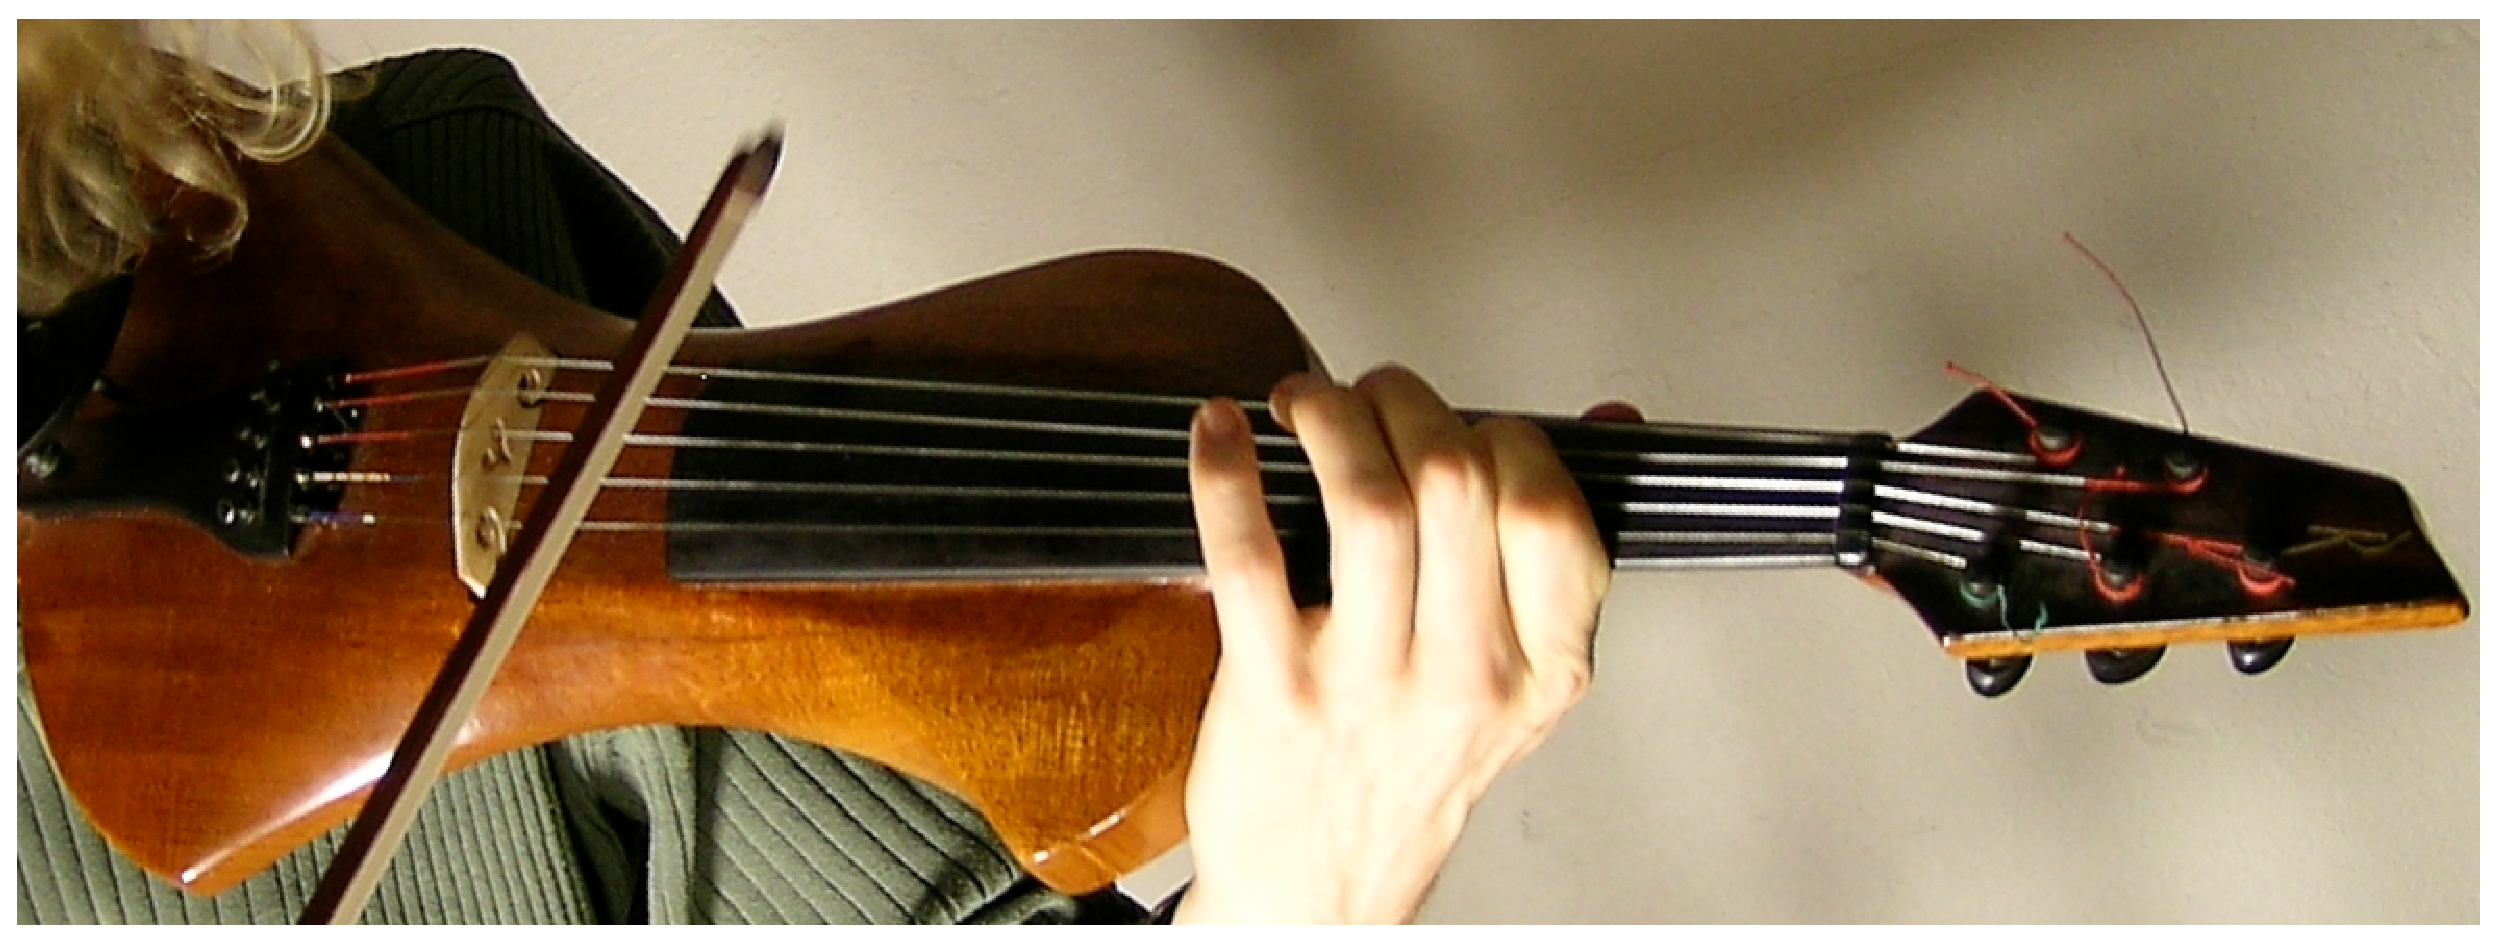
\includegraphics[width=0.4\linewidth]{img/evg-2}
  \caption{The Electric Viola Grande, an electronically amplified viola built by Swedish instrument-maker Richard Rolf.}
  \label{fig:evg}
\end{figure}
%\vspace{1cm}

\subsection{Drive}
\label{sec:drive-2003}

\begin{wrapfigure}{r}{0.45\linewidth}
  \begin{minipage}[h]{\linewidth}
    \begin{flushright}
      \musicannot{Drive\\
        \emph{for Electric Viola Grande and computer}\\
        Composed \& premiered in 2002\\
        Commissioned by and dedicated to Henrik Frendin}
    \end{flushright}
  \end{minipage}
\end{wrapfigure}

%%% Local Variables: 
%%% mode: latex
%%% TeX-master: "../ImprovisationComputersInteraction"
%%% End: 

\emph{Drive} is a composition for \index{Electric Viola Grande}\index{EVG}Electric Viola Grande (EVG)\footnote{The Electric Viola Grande is a custom made, electronically amplified five stringed viola. It was built by Swedish instrument-maker Richard Rolf on commission from Swedish violist Henrik Frendin.}  and computer commissioned by Swedish violist Henrik Frendin for his Phono Suecia recording \emph{Viola con Forza}. \footcite{frendin04} Within the frame of the composition the performer has much freedom to shape the piece in a way that he or she sees fit in order to fulfil the larger structural idea of the composition: a dominant to tonic cadence. The synchronisation between the computer and the performer is achieved by employing the widely used space-bar-piece paradigm:\footnote{I heard this term used for the first time by Sean Ferguson (see \url{http://www.cirmmt.mcgill.ca/People/ferguson}). In the mid 1990s, when it started to become practical to use computers in live performance, a large number of compositions were produced where someone other than the performer(s)---usually the composer---interacted with the computer using the computer keyboard. Each touch of the space bar (or any other key of choice) started the playback of the next pre-prepared sound file or changed the settings (the preset) for an effect or a synthesiser or whatever the next `event' required. It is still a very common mode of interaction in the \index{electro-acoustic music}electro-acoustic music community.} the computer is guided through the different sections of the form of the composition by means of `cues' (pressing the space bar).\footnote{The cue may of course come from any kind of control source from which a clear, noise-free, trigger can be generated such as a pedal pressed by the performer; a uniquely detected pitch in the audio signal; a change of volume; etc.} For every cue (a total of six in the piece) the computer adjusts its internal tempo based on the time lapse since the last cue. In other words, the computer part with its associated `player' and `listener' is progressing at its own pace, occasionally adjusted to the performer's tempo. Although the significance of time in interactive systems will be treated in more depth \hyperref[sec:time-interaction]{in Section \ref*{sec:time-interaction}} the difference between this kind of time based system such as \emph{Drive} implements and a purely event based system should be noted. Whereas the former, in its conception of time, displays some notion of memory or history, though only in a very limited sense, a purely event-based system, with no regard to time, responds to each trigger individually, similarly to how most computer text editors will respond to the trigger \emph{letter `T' pressed} in the exact same way regardless of what came before it, or how synthesiser keyboards respond to the \emph{MIDI note 64} message uniformly disregarding context (see \autoref{fig:serial}). In a very simplistic way the computer part for \emph{Drive} has its own forward motion and its own tempo. It moves in parallel with the performer rather than \emph{only} as a result of a stimulus, and updates its motion and its state according to the cues it receives (see \autoref{fig:parllel}). It is its motion that constitutes its memory and it is the altered tempo that affects subsequent events.

\begin{wrapfigure}{r}{0.55\linewidth}
  \centering
  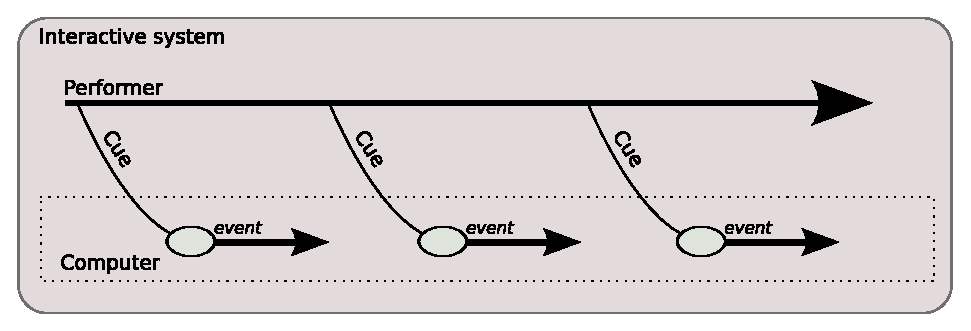
\includegraphics[width=0.95\linewidth]{img/serial}
  \caption[Scheme of a simple interactive system without memory.]{An interactive system with a performer providing the computer (synthesiser, dishwasher, etc.) with singular cues. The (computer) system is agnostic to past cues and events and reacts only to the current or most recent event, i.e. it has no memory as such.}
  \label{fig:serial}
\end{wrapfigure}
Apart from the cues to guarantee synchronisation between the performer and the computer, another more dynamic layer of \emph{harmonic} interaction is active throughout the piece. The computer part resonates with particular frequencies, in terms of both when and how to manipulate the sound of the EVG and when and how to generate new material; a virtual resonance that is used to expand the spectral and timbral range of the instrument. The resonating frequencies are subject to constant change following the composed viola part as well as following the tempo as altered by current and prior cues. Thus it constitutes a sonic layer of communication between performer and computer. If they drift apart in time, there will be less, or substantially different, sonic interaction (an effect the first version of the score already allowed for).

\begin{wrapfigure}{l}{0.55\linewidth}
  \centering
  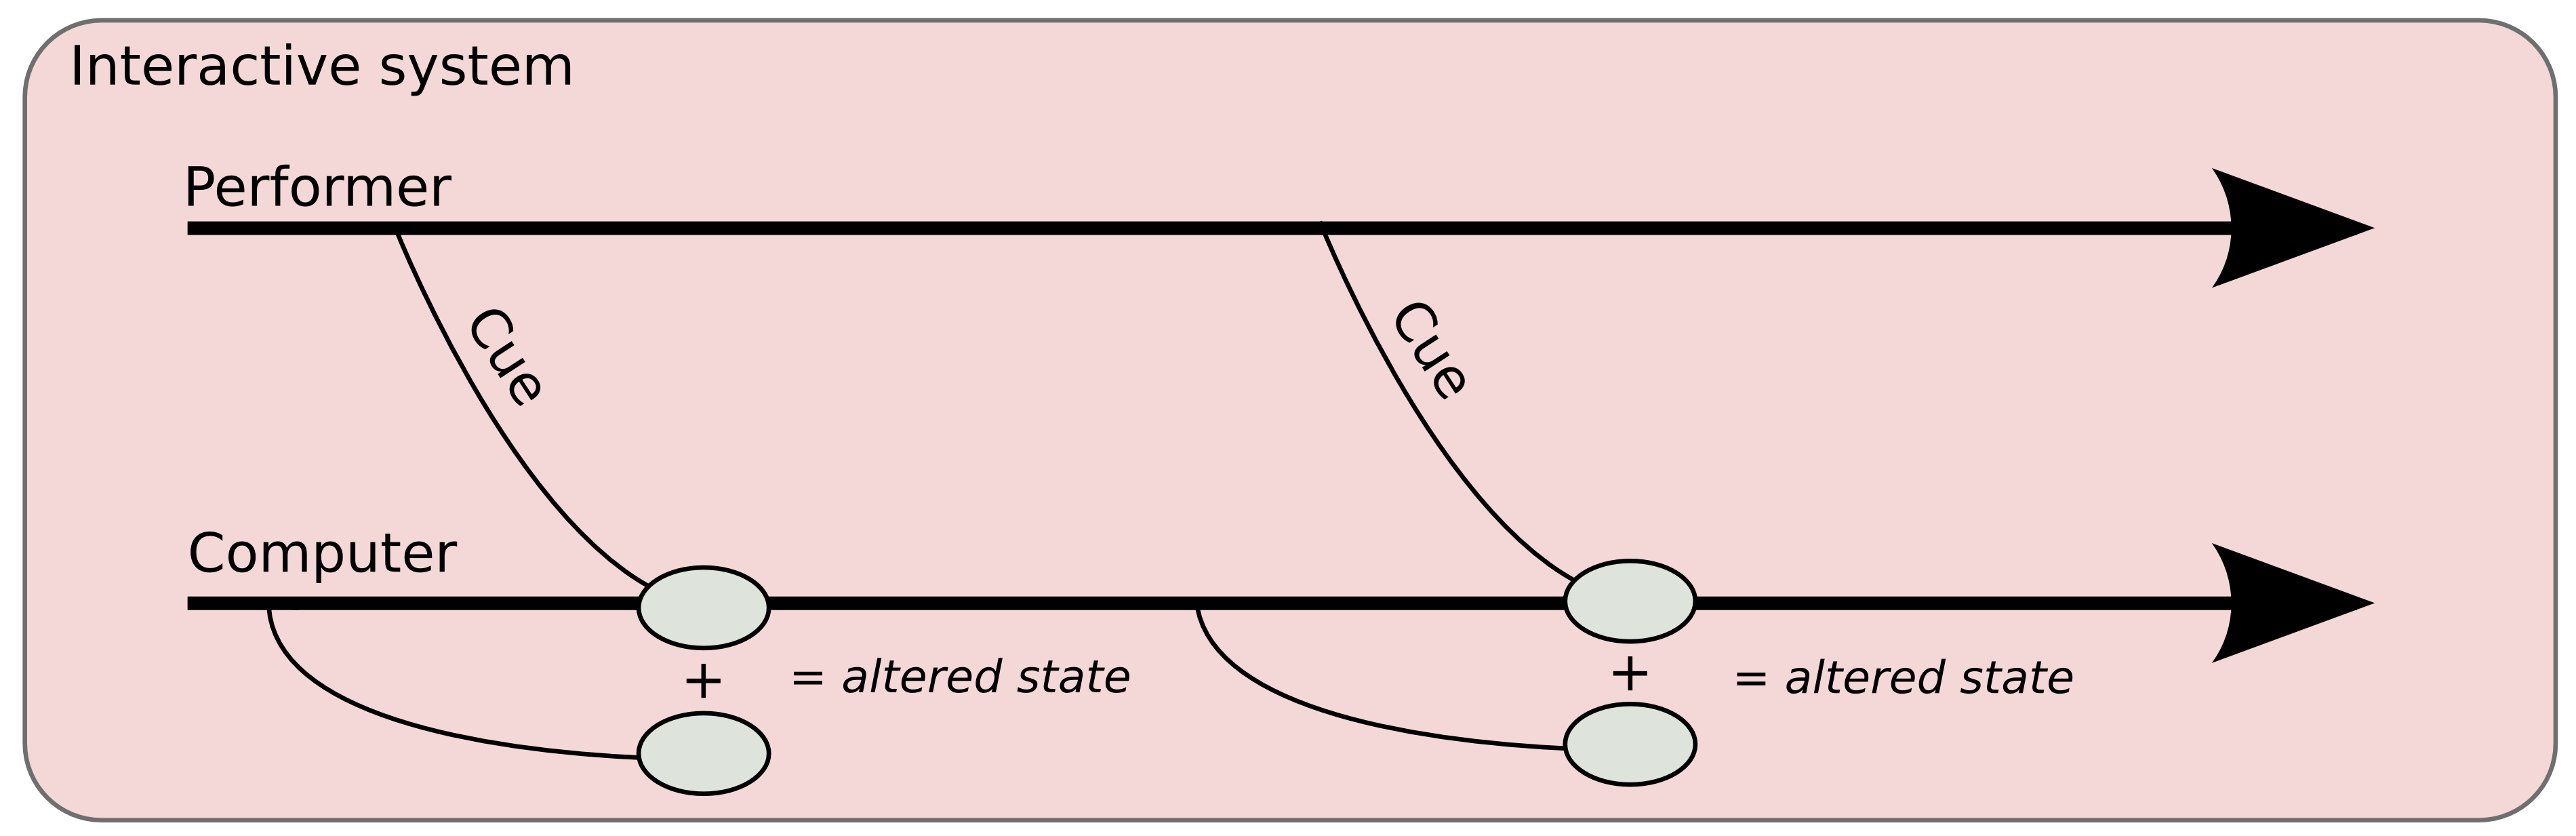
\includegraphics[width=0.95\linewidth]{img/parallel}
  \caption[Scheme of a simple interactive system with memory.]{An interactive system with two players in parallel with a simple implementation of memory. The altered state is a result of the most recent cue \emph{and} past cues and events.}
  \label{fig:parllel}
\end{wrapfigure}
Finally, \emph{Drive} is a composition in which the interaction between myself, as the composer, and Henrik Frendin, as the interpreter, is mediated through an open-ended score. In an ongoing negotiation we each have to question our respective views and personal wishes and open ourselves up to the other's point of view and trust that that view is `genuine'. One result of these negotiations is how the piece was originally conceived of as one that could be played by Frendin alone, that is, without my participating in the performance. Owing to a multitude of factors, however, one being that Frendin preferred me to perform with him, I have taken part in all performances of \emph{Drive}, which has obviously influenced how the piece has developed in the course of the performances and how the idea of interaction has changed from a performer-centred view to a distributed array of interconnected `players'. But it also had more radical consequences that have resulted in a deconstruction (though not so much in the philosophical meaning) not only of the original understanding of \emph{Drive} as a composition (rather than a \useGlosentry{glos:work_in_movement}{work-in-movement}), but of my own role as composer. My performances with Frendin have grown to engendered new positions for both of us. If formerly I assisted Frendin in the `performance of compositions' we now approach our venture with much more distributed roles, hovering in the crevices between composition, improvisation, performance and mixing. Hence, \emph{Drive} initiated another aspect of the dismantlement of the \index{Self}Self possible only if one is \emph{willing} to give up the \index{Self}Self.

Although this project was initiated prior to the studies in \emph{Negotiating the Musical Work}, the project I share with guitarist Stefan \"{O}stersj\"{o},\footcite{frisk-ost06} it nevertheless anticipated certain aspects of collaborative music making, ideas that would later be formalised.

\subsection{etherSound}
\label{sec:ethersound-2003}

\begin{wrapfigure}{r}{0.4\linewidth}
  \begin{minipage}[h]{\linewidth}
    \begin{flushright}
      \musicannot{etherSound\\
        \emph{for improvising musicians, audience and mobile phones.}\\
        Composed \& premiered in 2003\\
        Commissioned by Miya Yoshida}
    \end{flushright}
  \end{minipage}
\end{wrapfigure}

%%% Local Variables: 
%%% mode: latex
%%% TeX-master: "../ImprovisationComputersInteraction"
%%% End: 


\emph{etherSound} is perhaps the most ambitious sub-project. It was commissioned in 2002 by curator Miya Yoshida for her project \emph{The Invisible Landscapes} and was realised for the first time in August 2003 at \emph{Malm\"{o} Art Museum} in Sweden.\footcite[Yoshida's PhD thesis includes a chapter on \emph{etherSound}.][C.5, \pno 165]{yoshida06} Since then it has been performed on several occasions in Sweden, Denmark, the UK and the USA. The principal idea behind \emph{etherSound} is to create a vehicle for audience collaboration in the shape of an `instrument' that is playable by anybody who can send SMS (Short Messages Service) messages. As an interactive system \emph{etherSound} takes input in the form of these SMS messages and creates `message-scores', then transforms them to short electro-acoustic `message-compositions', each one lasting from about fifteen seconds to two minutes. The length of the event depends on the relative length and complexity of the message text. Hence a short message will be more likely to generate a shorter message-composition than a long message, but a short message with a couple of words with inter-punctuation may render a longer message-composition than a long message containing only gibberish, but the message-composition's inherent sonic complexity may be increased by a more complex message. The length and complexity of the message-composition is, however, also governed by previous messages and in that sense it also exhibits, just like \emph{\hyperref[sec:drive-2003]{Drive}}, a rudimentary kind of memory or parallelism with its users. \emph{etherSound} is an effort to move the initiative of making and distributing sounds from the composer/musician to the listener and it can take on different shapes (a performance environment, sound installation, composition tool, etc.) \hyperref[sec:summary]{As already mentioned}, it investigates aspects relating to the \index{Self}Self and to the roles of composer, performer and listener and it may perhaps best be described as an environment that allows for interaction between different agents on different levels simultaneously. The wish to participate is intended to be the only requirement for participation: The audience is used (exploited?) to supply that which the computer does not have (and which we are not likely to be able to model within a computer for another few years yet)---intentionality. No matter the sophistication of the interface---or the lack thereof---no matter the mapping between cause and effect, the `message-composition' is brought to life because someone intended to bring it to life, and therefore intended it also in a phenomenological sense.

This and other aspects of audience participation are an important part of \emph{etherSound}. It may distort not only the \index{Self}Self, but also the way we understand the roles of the other agents involved in the production of this event.\footnote{In relation to the discussion of the \index{ontology}ontology of the musical work which is being probed in the paper, see \cite{frisk-ost06-2}} The transformation from private to public (an SMS emanating in the private sphere from a privately owned mobile phone results in a publicly perceptible sound event) prepares the way for a different sensation of space and an auspicious and dynamic impression of participation as creativity. This shift from private to public is related in this thesis to the central idea of `the giving up of the \index{Self}Self' (the private) as a first step towards interaction (the public) on equal terms. The problematic relation between user \emph{control} through interaction---the participant's chance to discriminate his or her input from other input, i.e. the transparency of the system---and interaction as `dialogue', is furthermore made tangible in all versions of \emph{etherSound}.

Apart from the many performances of \emph{etherSound} I have also used it to produce a recording released and included with this project featuring, apart from myself, Peter Nilsson on drums and percussion. The idea of recording an interactive sound installation may, to say the least, appear as counter productive, for no medium appears less interactive than the CD. The CD, however, is an attempt to reconnect to an earlier performance of \emph{etherSound} that took place on 8 May, 2004 at \emph{Jeriko} in Malm\"{o}, Sweden and is no less interactive than any performance version of it, but it is interactive in different ways. In the recording we are interacting with the absent participants whose intentionality has been preserved in their contributions. We are using the `recorded' SMS messages along with their time information to `play' back an `electro-acoustic' track with which we improvise. The messages appear in the exact same order and at the exact same relative time position as they were received in the concert and in that sense this recording is a mirror image in time of that evening. Those who participated in the concert also participate in this recording.\footnote{At http://www.henrikfrisk.com/ethersound participants in the event may register with their phone number in order to be credited for their contribution (anonymously if they so wish).}

\subsection[Repetition\ldots]{Repetition Repeats all other Repetitions}
\label{sec:negot-music-work}

\begin{wrapfigure}{r}{0.45\linewidth}
  \begin{minipage}[h]{\linewidth}
    \begin{flushright}
      \musicannot{Repetition Repeats all other Repetitions\\
        \emph{for ten-stringed guitar and computer}\\
        Composed \& premiered in 2006\\
        Commissioned by and dedicated to Stefan \"{O}stersj\"{o}}
    \end{flushright}
  \end{minipage}
\end{wrapfigure}

%%% Local Variables: 
%%% mode: latex
%%% TeX-master: "../ImprovisationComputersInteraction"
%%% End: 

This collaboration with the Swedish guitarist Stefan \"{O}stersj\"{o} is an example of a project in which at the outset interaction in the widest sense was allowed to play a major part. The process is fairly well documented in our two co-written papers \citetitle{frisk-ost06} and \citetitle{frisk-ost06-2} \nocite{frisk-ost06,frisk-ost06-2} and it was while working with \emph{Repetition\ldots} that the idea of a radically open work type, the \useGlosentry{glos:work_in_movement}{work-in-movement}, crystallised. One of the conditions that allowed for the development of this openness was the disassembly of the hierarchies attached to the roles of composer and performer. These hierarchies rest on a division of labour in the field of musical practice, and this ``split in conception between what is seen as primary [notation] and secondary [sound] aspects of musical organisation leads to a split between composer and performer, between composition and interpretation and the gradual devaluation of non-notable formations''.\footcite[35]{wis96} It was a tear in the fabric on which, prior to the ``increasing domination of notation'',\footcite{wis96} the practice of `\useGlosentry{glos:musician}{musician}' rested. In part this sub-project became the beginning of the attempt at re-uniting the different aspects of the `musician', necessary because the collaborative process we had set in motion was irreversible. There was no way back; it was impossible to return to producing \emph{the score} to be \emph{interpreted}. For so many years I had tried so hard to incorporate aspects of my improvisatory activities in my composition work whereas the solution instead was the `decomposition' of the very act of producing music. By giving up compositional control and hence giving up part of the \index{Self}Self and replacing it with an interactive negotiation in the form of a collaboration the process was possible.

\begin{wrapfigure}{r}{0.5\linewidth}
  \begin{minipage}[h]{\linewidth}
    \begin{flushright}
      \musicannot{
        Repetition Repeats all other Repetitions, Symphonie Diagonale\\
        \emph{for ten-stringed guitar, computer and video projection}\\
        Composed \& premiered in 2007\\
        Prepared in collaboration with Stefan \"{O}stersj\"{o}}
    \end{flushright}
  \end{minipage}
\end{wrapfigure}

%%% Local Variables: 
%%% mode: latex
%%% TeX-master: "../ImprovisationComputersInteraction"
%%% End: 

Considering \emph{only} the musical notation of the score,\footnote{See the book homepage for a score excerpt.} the first impression may be that \emph{Repetition\ldots} belongs precisely to the tradition of compositions that \citeauthor{wis96} is criticising, a tradition where ``the score is seen as normative on the musical experience.'' The first version of the score bears evidence that, at the time, the idea of the work-in-movement had not been fully incubated. It also points, however, to the difficulty in communicating a radically open work. Given the way \emph{Repetition\ldots} has developed, the written instructions (i.e. the notation) are subordinate, yet important, to the higher level structures of organisation: the interaction between, in this case, myself and Stefan has become the work identifying aspect. But neither I nor Stefan are important: if someone else picked up \emph{Repetition\ldots} the interaction and negotiation itself would be the aspect to focus on. This obviously calls for a different conception of the score, an augmented score that apart from the notation also includes other kinds of instructions in other kinds of media.

Together Stefan and I have produced and performed three different versions of this piece. The third version take account of the ideas that were developed from the experiences of the two first versions, giving the performer a much higher degree of freedom. Future versions should be further developed and even more interactive making use of the \hyperref[sec:timbremap]{\emph{timbreMap}} \index{real-time}\index{time!real-time}real-time analysis tool. 

\newpage

\subsection{libIntegra}
\label{sec:libintegra}

\begin{wrapfigure}{r}{0.4\linewidth}
  \begin{minipage}[h]{\linewidth}
    \begin{flushright}
      \musicannot{IntegraBrowser\\
        \emph{Offline browser for the Integra XML\\documentation format.}}
    \end{flushright}
  \end{minipage}
\end{wrapfigure}

%%% Local Variables: 
%%% mode: latex
%%% TeX-master: "../ImprovisationComputersInteraction"
%%% End: 

Integra\footcite{integra-web} is an EU Culture 2000 pan-European artistic and scientific project. One of the goals is to develop a composition and performance environment for sharing live music technologies. One part of that environment is the Integra library (\emph{libIntegra}), the development of which I have participated in. The overarching goal of the scientific branch of Integra is to produce a set of \index{software}software tools that allows many musicians to work interactively on several different kinds of collaborative projects in a way that has not been possible earlier.

\emph{libIntegra} allow for a standardised way of representing and storing parameter spaces for multi-media modules.  One of the things this allows for is seamless interchange of units of \useGlosentry{glos:dsp}{DSP} processing (\index{software}software or hardware based) within a given context. A performer who wants to improvise with an environment that requires a Yamaha DX7 synthesiser may simply substitute the hardware with a \index{software}software representation of the same synthesis model. As long as the environment, and the modules within it, complies with the Integra standard the exchange is transparent from the user's point of view. The library is also able to interface with a centralised database and versioning server making possible interaction on any kind of content that the database and the library can represent and in that sense it is a \index{software}software representation of the very idea of the musical work as a result of distributed actions in continuous interaction: the \index{software}software version of the \emph{work-in-movement}. The various parts of the libIntegra \index{software}software development project (the IXD file format, the database, the library and the bridges) allow for seamless and integrated documentation of many different kinds of musical works---scores, interpretations of scores, performances of scores, improvisations, improvisation environments, etc. \emph{libIntegra} also allows for interaction across computer platform boundaries and \emph{timbreMap} integrates with any other \index{software}software for which \emph{libIntegra} has support. Finally, one possible implementation of the notion of the augmented score (\hyperref[sec:negot-music-work]{see Section \ref*{sec:negot-music-work}}) is possible within the framework of the Integra class hierarchy and the corresponding XML file format (Integra eXtensible Data). Just like \emph{Repetition...}, \emph{Drive} and \emph{etherSound}, \emph{libIntegra} is a collaboration, but on a somewhat larger scale\footnote{Though Jamie Bullock and I are the main developers of the libIntegra \index{software}software, the project Integra has members from eleven countries and six universities and a total of ten research centres and five new music ensembles are involved.}.

\hypertarget{sec:target:libintegra-1}{It should} perhaps be pointed out that the Integra project in general has aims that, to a certain degree, appear to contradict those that I am advertising here, in particular how I am proposing to use the \emph{libIntegra} with regard to the project \emph{Repetition\ldots}. For example, \emph{work preservation} and \emph{sustainability} are central aspects of the Integra project, as stated and explored in the two papers \citetitle{frisk-bull07} and \citetitle{frisk-bullock08}.\footcite{frisk-bullock08} Both of these concepts are rooted in the wish to archive and preserve works of art in one particular state in order to recreate them  as authentically as possible, that is, as close as possible to how they were once preserved. Those aims do indeed seem to counteract the concept of the \useGlosentry{glos:work_in_movement}{work-in-movement} which is primarily concerned with change and difference.

Owing, however, to the generic nature of the representations in the different parts of \emph{libIntegra} I found it possible to use the framework, unaltered, for my own purposes. A concept such as \emph{preservation} is, in the case of a versioned database, also an opening for non-preservation, development and sharing. In the Integra database no record can be easily altered, and any alteration results in a new record which inherits all the relations and properties of the earlier one. Additionally, the possibility of storing a local version of any set or subset of database objects, each of which may represent a \useGlosentry{glos:dsp}{DSP} module, a work instruction, a person, a building or any other kind of data type in the object oriented hierarchy of database classes, allows for local additions and alterations independent of any changes occurring on the server database. A representation of a musical work in the Integra database is less centred on \emph{notation} and more focused on \emph{relations} and \emph{differences}. It is a distributed though interconnected array of containers of information that by its nature of representation does not discriminate between the kinds of music it represents---the advantage of notational forms over improvisatory should decrease. It also allows for interaction and collaboration and in the context of the idea of \index{interaction!as difference}\index{interaction-as-difference}interaction-as-difference the versioning of the data is significant because it is only if the alteration, the difference induced, leaves the `original'---which may itself be an altered copy---intact that the difference may be traced. I believe that libIntegra may provide for a framework in which the \index{ontology}ontology of the musical work may be described, and, eventually, visualised in a meaningful way, in particular for the kind of works that do not lend themselves well to standard musical notation (such as improvisatory and collaborative works).

Finally, although \emph{libIntegra} is part of the larger Integra project, the code is licensed under the \citetitle{GNUGPL} by myself and Jamie Bullock. In other words it is possible for the framework to take off and continue developing outside the range of the goals and ideologies of the Integra project.

\section{Artistic practice and interaction---Summary}
\label{sec:music-pract-inter}

By taking a broad view on interaction in music (such as stating that programming is interactive and that all music listening activity is interactive) there is an obvious risk that everything becomes interaction, which, in fact, is the same as saying that nothing is interaction. Now, the opposite would clearly be equally destructive: to employ a rigid definition of interaction and shutting out that which does not fit the program. Is it possible to look at \emph{qualities} of interaction or interactive \emph{intensities} and thus avoid the delusive classifications? Or, if we look at interaction from the inside, perhaps it is possible to find the prerequisites for each type of interaction, its particular needs. Below I will attempt to map the sub-projects in different modes of organisation based on different kinds of criteria with the primary purpose of showing the multiple interactive possibilities within any kind of musical practice with the computer. 

Though neither an exhaustive list of possible interactive contexts, nor a complete description of the interaction in these projects, an intermediary categorisation of types of interaction explored within the different sub-projects, based on \emph{who} is interacting, may be outlined:

\begin{itemize}

\item \textbf{Musician-Computer Interaction}
  \begin{itemize}
  \item Performer-computer interaction in score-based works   (\emph{Drive}, \emph{Repetition...}, \emph{timbreMap})

  \item Performer-computer interaction in improvised works (\emph{solo improvisations}, \emph{timbreMap})

\item Audience-computer interaction (\emph{etherSound})

  \end{itemize}

\item \textbf{Musician-Musician Interaction}
  \begin{itemize}

  \item Composer-performer interaction (\emph{Repetition...}, \emph{libIntegra})

  \item Performer-performer interaction (\emph{etherSound}, \emph{Drive})

  \item Performer-audience interaction (\emph{etherSound}, \emph{libIntegra})
  \end{itemize}
\end{itemize}

% \begin{wrapfigure}{r}{0.6\linewidth}
% %\begin{figure}[!htb]
%   \centering
%   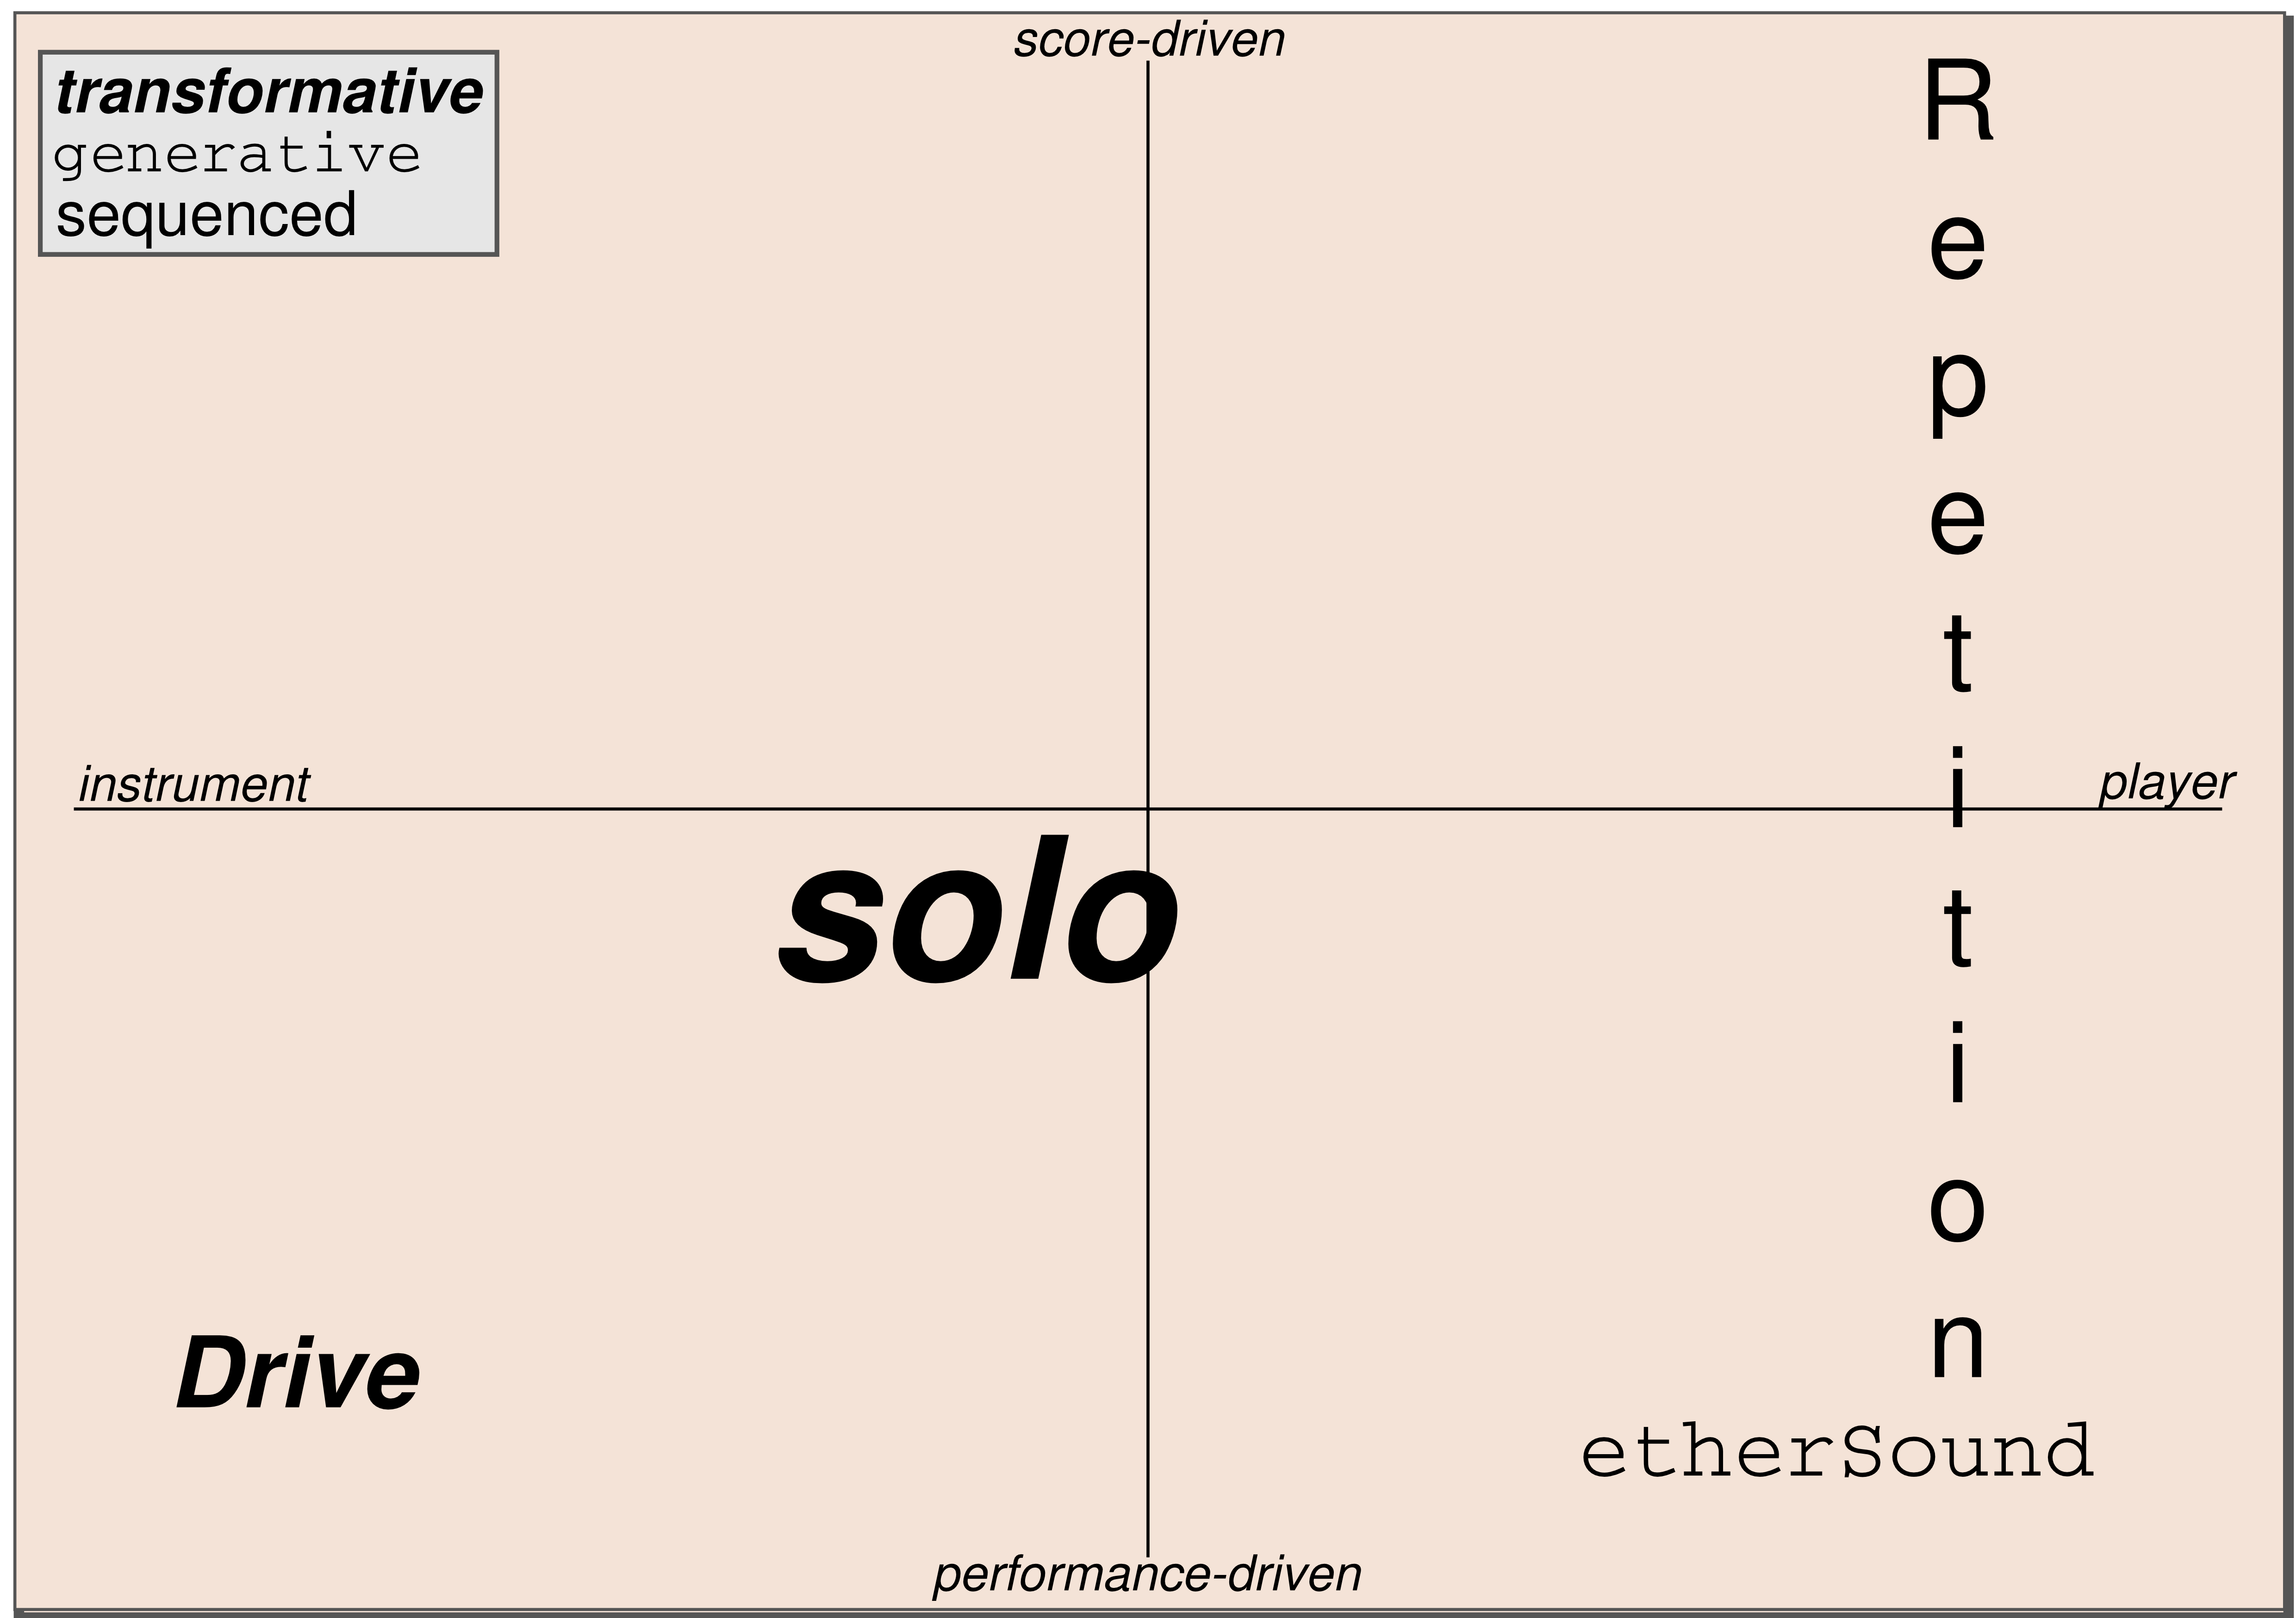
\includegraphics[width=0.97\linewidth]{img/interact-class}
%   \caption[A map of the artistic contents of the project.]{The approximate position of the artistic content in the three classification dimensions suggested by Rowe\footcite[5--8]{rowe}. The font \textit{type} is used in the graph to discriminate between the different response methods. The font \textit{size} is used to indicate the stability of the project in relation to the categories. For example, in my saxophone-computer improvisations (here depicted \emph{solo}) I use a large number of interactive techniques and programs, hence the font size is large, whereas \emph{etherSound} is fairly well categorised as a generative, performance-driven player---and is thus represented by a relatively small font size.}
% \label{fig:interact-class}
% %\end{figure}
% \end{wrapfigure}
As with any clearly delimited categorisation, the categories themselves risk producing more questions than answers (although that should not be seen only as a problem). Each kind of interactive context has its own set of requirements. A performer playing a scored piece for instrument and computer, such as \emph{Drive}, has different needs and expectations than does an improviser, and all performers do not have the same anticipations. Improvising \emph{with} a computer as a saxophonist is in every respect different from improvising \emph{on} the computer. 

%\newpage
In his book \emph{Interactive Music Systems}, composer, programmer, and researcher Robert \citeauthor{rowe} makes a classification of interactive music systems that may prove useful to help interrelations between the interactivity at play within these four sub-projects---containers of musical practice---in the context of the larger scope of the research project as a whole. I will apply these classifiers in an attempt to dismantle the concepts involved, as part of the research. For \citeauthor{rowe} the ``motivation for building such a set of classifications is not simply to attach labels to programs but to recognize similarities between them and to be able to identify the relations between new systems and their predecessors.''\footcite[6]{rowe} Although \citeauthor{rowe}, at least here, is more concerned with the actual \index{software}software in the system, categories such as those presented are also useful also in artistic work, for much the same reasons,not primarily because computer programming may be a truly artistic process, but because a methodological tool such as this (it is a classification method) allows for connections between disparate  projects to be identified in ways not possible without it.

\begin{figure}[!htb]
  \centering
  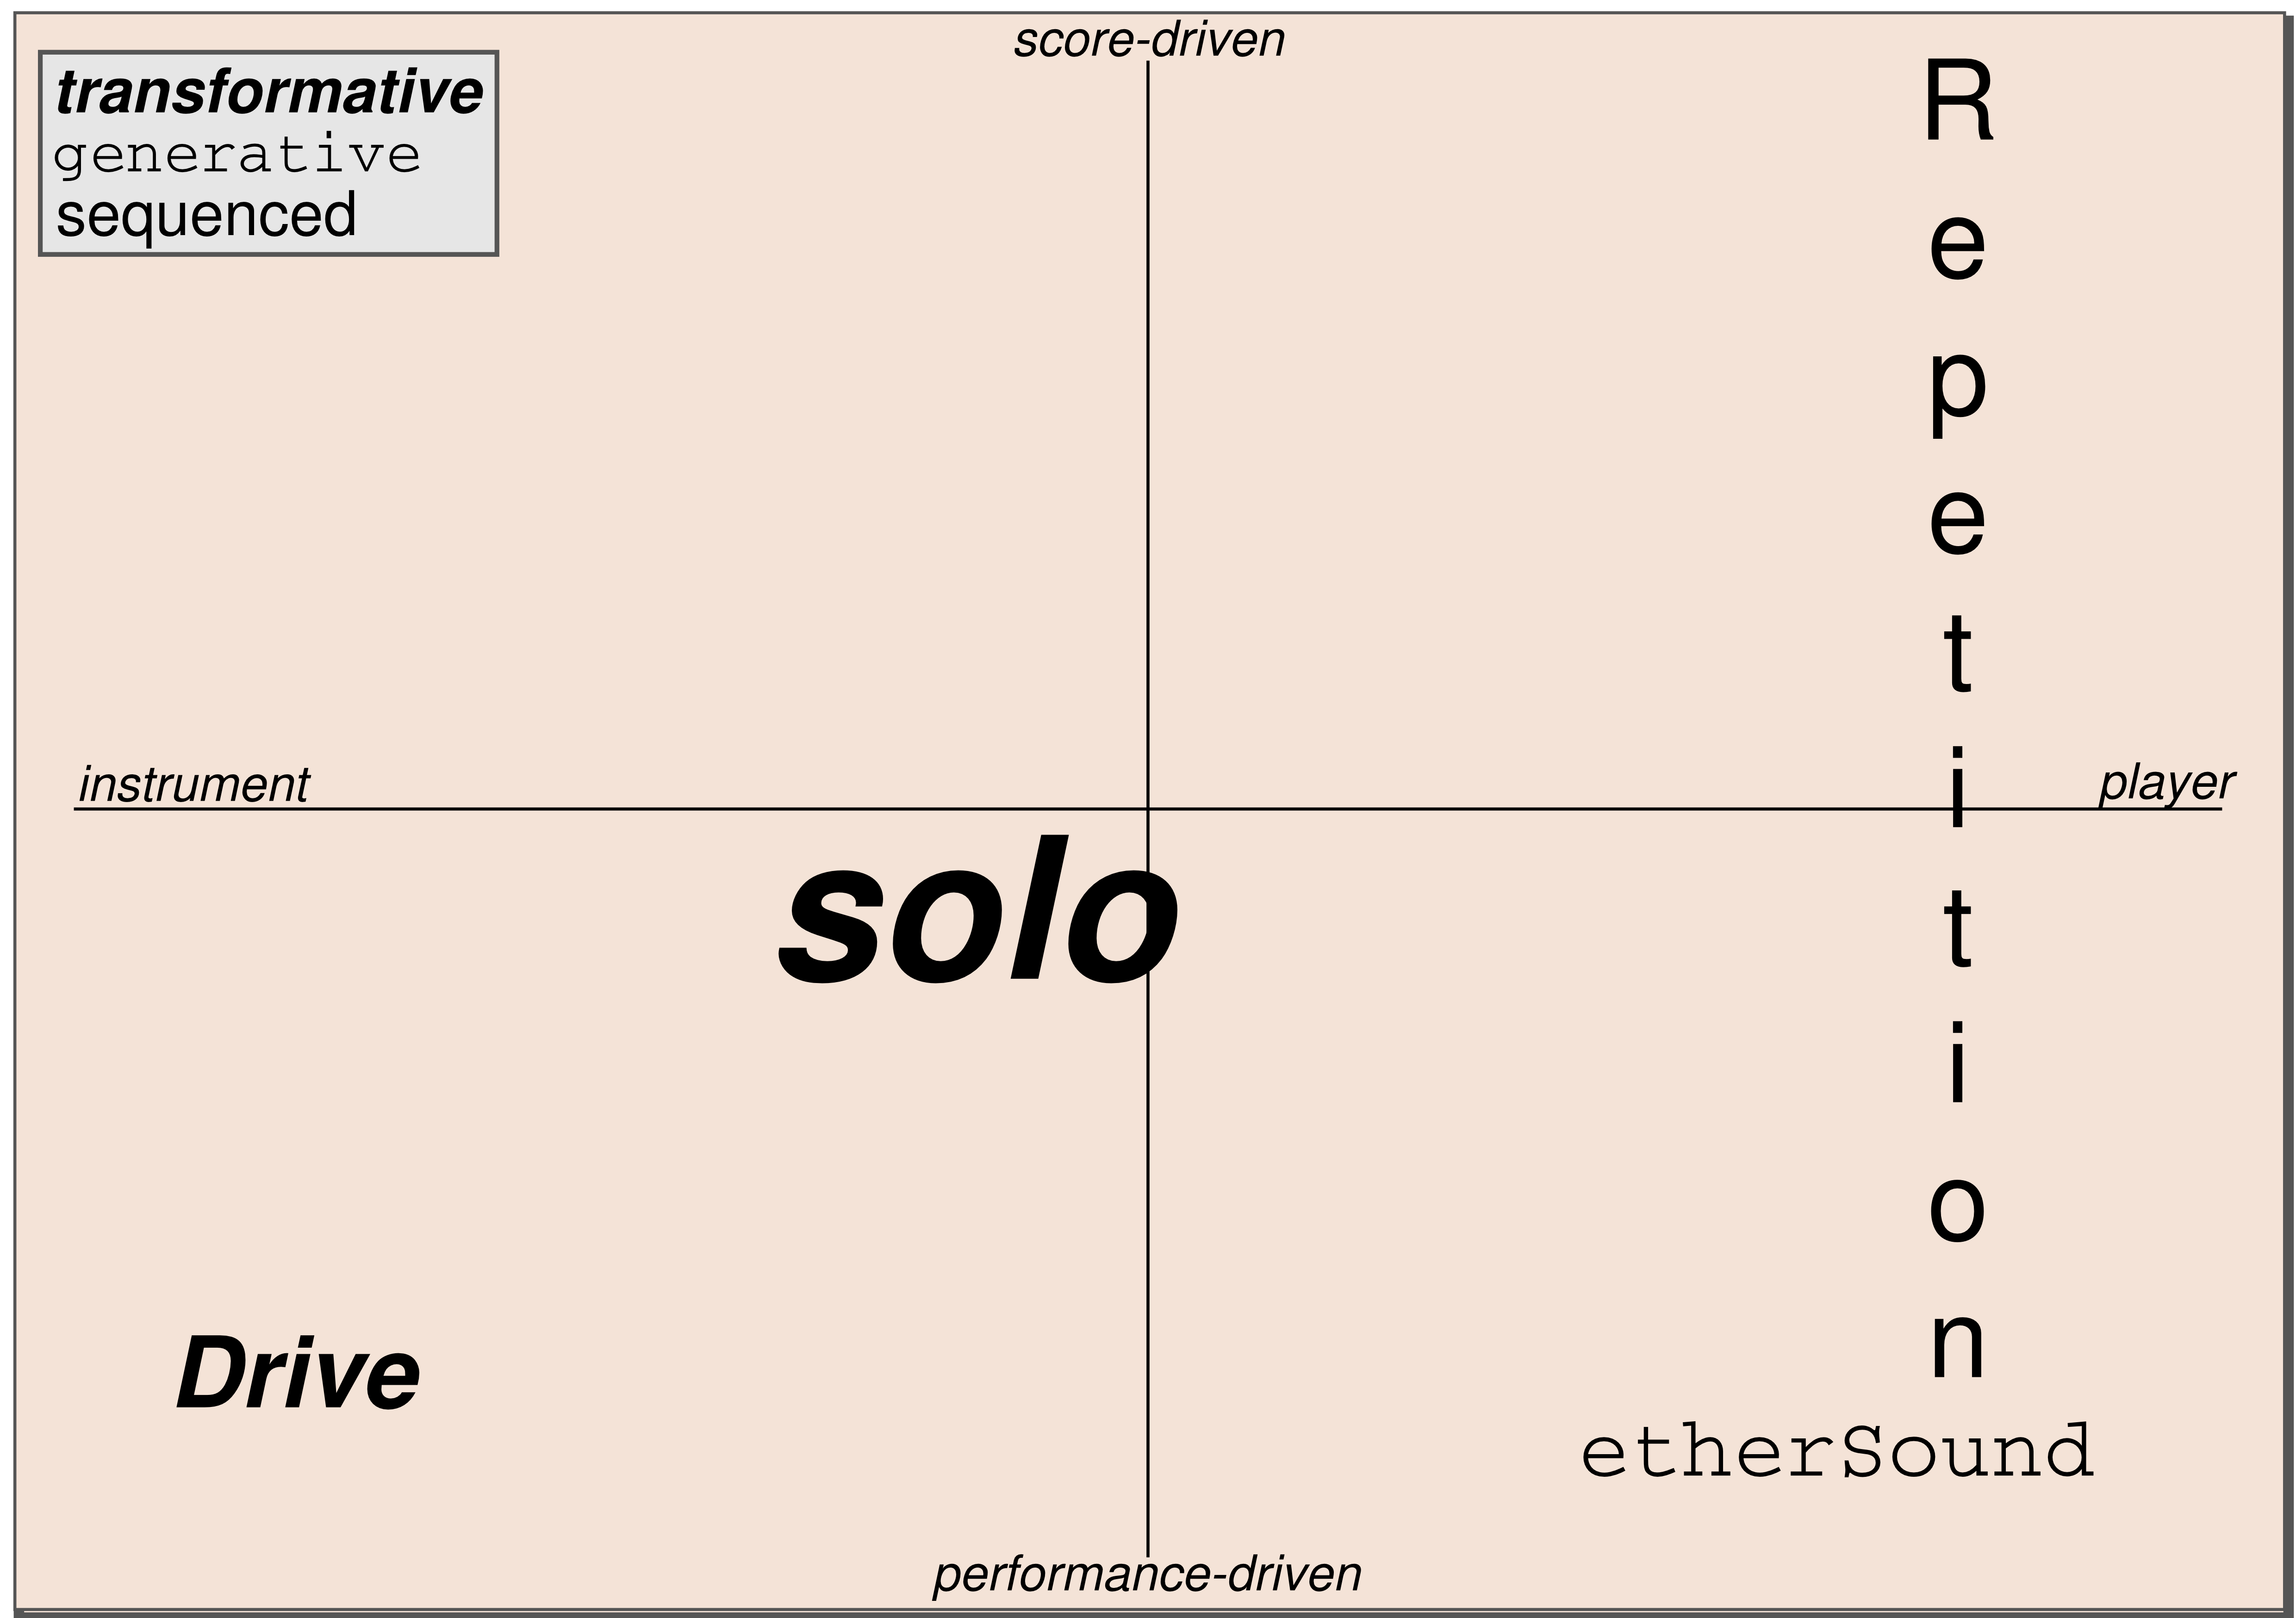
\includegraphics[width=0.9\linewidth]{img/interact-class}
  \caption[A map of the artistic contents of the project.]{The approximate position of the artistic content in the three classification dimensions suggested by Rowe\footcite[5--8]{rowe}. The font \textit{type} is used in the graph to discriminate between the different response methods. The font \textit{size} is used to indicate the stability of the project in relation to the categories. For example, in my saxophone-computer improvisations (here depicted \emph{solo}) I use a large number of interactive techniques and programs, hence the font size is large, whereas \emph{etherSound} is fairly well categorised as a generative, performance-driven player---and is thus represented by a relatively small font size.}
\label{fig:interact-class}
\end{figure}


As for the classification system, it is ``built on a combination of three dimensions, whose attributes help identify the musical motivations behind types of input interpretation, and methods of response''.\footcite[6]{rowe} That is, the way the system handles its input and how it generates its output and, according to \citeauthor{rowe}, the classifiers will provide us with a terminology which can be used to ``distinguish and draw relations between interactive programs''.\footcite[7]{rowe} 

%Though \citeauthor{rowe} uses the classifiers primarily for computer \emph{programs} I find them useful also for the point at issue.\footnote{This is likely to be because most of these projects feature at least one `program', specially designed for the purpose, even though it may only consist of a simple Max patch \parencite{max}.}

The categories in the three dimensions are:\footcite[These categories are clearly outlined in][and all the citations below are taken from p.7--8]{rowe} 

\begin{enumerate}
\item \emph{Score-driven} systems versus \emph{Performance-driven}, i.e.  systems that range from ``programs that use predetermined event collections'' (a score), to those that ``do not anticipate the realization of any particular score''.

\item \emph{Transformative}, that apply a transformation on some existing material, \emph{Generative}; that generates material from ``elementary or fragmentary'' source material (a scale or a chord), or \emph{Sequenced}, that ``use pre-recorded music fragments'', response methods.

\item \emph{Instrument} versus \emph{Player} paradigms, where the former is primarily ``concerned with constructing an extended musical instrument'', and the latter with constructing ``an artificial player'' that performs some material.
\end{enumerate}

These categories, employed in the artistic work in this project, are visualised in Figure \ref{fig:interact-class}, but it should be noted that, as is generally pointed out by Rowe,\footcite[6]{rowe} these are not fixed positions but possible starting-points. Also, as we shall see in the discussion on \emph{etherSound}, it may be very difficult to determine exactly what constitutes a `score' and, if a piece may be said to have a score which is represented in the interactive system, can it still be categorised as a \emph{performance-driven} system rather than as a \emph{score-driven} system? At any rate, the presented categories allow us to get a topological overview of the included projects' relation to different types of interactive systems in music. Further, as was briefly mentioned above, using these categories is a method adopted for reflection and presentation, not construction---I did not pre-conceive the respective projects' positions on this map. Though I did have an idea of what kind of artistic content should be included when I started this research project, none of these projects were created with the primary goal of \emph{illustrating} a method of interaction.\footnote{In a way I was surprised to see how scattered these projects were on the category map. I would have anticipated a tighter focus.} For better or worse, the only difference between my work in this artistic field within the scholarly frame of my PhD studies and the work done outside it is the added layer of reflection and the possibility to work things through more thoroughly. And, in the nature of my artistic practice---and I believe many others'---despite how rigorously a project is planned in advance, in the course of action it is bound, and should be allowed, to develop in unforeseen ways.

The one piece that most clearly lends itself to these categories is the first version of \emph{Repetition Repeats all other Repetitions}. The only possible interaction between the performer and the computer is mediated through a foot pedal---whether the pedal is down or up is the only information that the computer is `listening' to. In the other direction, as a result of the pressed pedal, there is a very complex flow of different types (classes) of information that the performer is expected to respond to: visual feedback from the computer screen on stage, physical (tactile) feedback from the pedal, auditive feedback in the sounds played back on the computer, all of which influence how the performer performs the piece. In other words, something incredibly concise and limited such as the binary distinction between pressed pedal or released pedal gives rise to a plenitude of messages of other kinds. This situation---the inconsistency between input and output---was what, at the outset of this research project as a whole, as well as at the beginning of the composition process of this particular piece, I thought of as a problem for which alternative solutions had to be invented: ``In our joint project we will attempt to avoid the kind of binary oppositions that require a clean control signal path (such as the pressing of a pedal) in the design of the interactive system''.\footcite{frisk-ost06} The foot pedal in this context is nothing more than a (non-musical) instrument to \emph{control} the computer part.

%\footnote{Compare to the discussion in Section \ref{sec:human-comp-inter} and Section \ref{sec:interaction} regarding the idea of interaction-as-control.}

In the theoretical realm the problem is the attempt to combine two radically different classes of information flow: one binary (pedal up/pedal down) and one continuous (primarily sound). The nature of the perceived response is opposite in quality to the nature of the stimulus.
%\footnote{This issue will be discussed more in the section on \emph{Interactive Music}.}
Yet, as music the piece works well,\footnote{Stefan has performed this version of the piece in Hanoi, Beijing, Malm\"{o}, Palo Alto, Seattle and Birmingham.} and I am pleased with the way the electronic sounds integrate with the guitar part. Perhaps in this piece the human-human interaction taking place in preparation for the project and Stefan's involvement in the process of composition in a way \emph{substitute} for the lack of \index{real-time}\index{time!real-time}real-time interaction? We are preparing a third version which will involve a more complex scheme of \index{real-time}\index{time!real-time}real-time interaction, not in order to prove the first version inferior (nor superior for that matter), but because it is in the nature of the piece to do several versions of it.

At the other end of the spectrum of my artistic work\footnote{\emph{Repetition...} features a (very) detailed score, and my solo work is entirely improvised; in \emph{Repetition...} I do not perform any part, but in my solo work I perform every part, and so forth.} lie my solo improvisations with computer---which on the map in \hyperref[fig:interact-class]{Figure \ref*{fig:interact-class}} are placed almost in the middle but employ a large number of different techniques---and I primarily look to achieve two things. (\textit{i}) Unity in sound (timbre) between the sounds produced acoustically and those produced electronically. This is not to say that I want the range of possible electronic sounds limited to saxophone sounds but that I look for a musical logic to the way the electronic sounds develop in relation to the saxophone sounds.\footnote{\hyperref[sec:timbremap]{See the section on \emph{timbreMap}} for further discussion on unity and sonic interaction. See also the \hyperref[sec:interraction-self]{chapter on interaction}.} (\textit{ii}) A level of interaction that is not constrained to a control interface---close to how George Lewis described a performance of \emph{Voyager} cited above (see \hyperlink{sec:target:personal-background-1}{Section \ref*{sec:personal-background}}). I too would rather have the computer surprise me than always to follow me:

\begin{squote}
In improvised music, improvisers often assert both personal narrative and difference as critical aspects of their work. For me, what Jerry Garcia called the ``anti-authoritarian'' impulse in improvisation led me to pursue the project of de-instrumentalizing the computer. If the computer is not treated as a musical instrument, but as an independent improviser, difference is partly grounded in the form of program responses that are not necessarily predictable on the basis of outside input. As we have noted earlier, Voyager's response to input has several modes, from complete communion to utter indifference. This seeming lack of uniformity is not necessarily correlated with ``lack of structure,'' as is so often expressed in the vernacular discourse of ``randomness.'' Rather, while tendencies over a long period of time exhibit consistency, moment-to-moment choices can shift unpredictably.\footcite[36]{lewis00}
\end{squote}

I think \emph{Voyager}\footcite{lewis92} is a great success as a framework for improvisation, as an interactive system, as an artistic expression that incorporates different modes of thinking about art and improvisation, and, for me, as a source of inspiration. The connection between that which is played by Lewis (and Roscoe Mitchell on the tracks that he appears on) and that which is performed by the computer is on some levels very clear yet without being obvious, and the way the musical gestures of the computer part are articulated has a distinct quality and resemblance to improvised music in a certain tradition. And this despite the fact that the computer is given no information about \emph{the sound} itself---the timbre. Only the pitch is fed to the computer.

There are obvious reasons for this choice of method of interaction in \emph{Voyager}: (\textit{i}) Pitch information may be quantified whereas timbral information can only be relative.\footnote{The definition of timbre from OED reads: ``The character or quality of a musical or vocal sound (distinct from its pitch and intensity) depending upon the particular voice or instrument producing it, and \emph{distinguishing it from sounds proceeding} from other sources''. The Oxford English Dictionary.  2nd ed. 1989. OED Online. Oxford University Press. (visited 14/11/2007). \url{http://dictionary.oed.com/cgi/entry/50252865} (my italics). It may be noted that, according to OED, two different sounds emanating from the same source---say a key click and a regularly played note on a saxophone---are not of different timbre. According to my understanding of timbre (and the English language) the last three words should be changed to ``from the same or other sources''.} Therefore pitch lends itself much more naturally to use as input in an algorithmic system of transformations.\footcite[Compare with \index{electro-acoustic music}electro-acoustic music composer and improviser Trevor Wishart's reasoning in][chap. 2]{wis96} (\textit{ii}) At the time \emph{Voyager} was created the technology for achieving and collecting information about timbre in \index{real-time}\index{time!real-time}real-time was very limited. (\textit{iii}) Even if information about timbre was to be extracted from the signal in \index{real-time}\index{time!real-time}real-time, the available \index{real-time}\index{time!real-time}real-time synthesis techniques were somewhat limited (and costly) at the time. (\textit{iv}) It may be a perfectly viable artistic choice to let the computer part have this quality of disruption, a quality of sound distinct from the acoustic sounds.

Musicologist Ingrid \citeauthor{monson96}, in her book on \index{interaction!musical}musical interaction in the jazz tradition, refers to the Charles Mingus-Eric Dolphy duet on the beautiful tune \emph{What Love}\footcite{mingus60} in which, according to \citeauthor{monson96}, it sounds ``as though they were having a very intense verbal argument''. Much later in the book, she returns to this recording and
the nature of the Mingus/Dolphy `argument':
\begin{squote} 
If I were to transcribe the notes and play them on the piano, they wouldn't sound very much like the conversation on the recording, for it is the relatively non-notable timbral and dynamic inflections produced by the players that are the principal means of signifying the iconicity.\footcite[208]{monson96}
\end{squote}
\hypertarget{sec:target:music-pract-inter-1}{When I listen to} \emph{Voyager}, I hear the playing of Lewis and Mitchell in a similar way: the particularity of that which is `said' is encoded in the \emph{sound} rather than the \emph{pitch}. This is, however, not how I perceive the voices of the computer part whose timbres are remarkably dull and static in comparison. To me, there is a perceptual breach between the electronic sounds and the acoustic sounds. 

\begin{wrapfigure}{r}{0.3\linewidth}
  \begin{minipage}[h]{\linewidth}
    \begin{flushright}
      \musicannot{Improvisations\\
        \emph{ for saxophone and computer}\\
        Performed in 2005}
    \end{flushright}
  \end{minipage}
\end{wrapfigure}

%%% Local Variables: 
%%% mode: latex
%%% TeX-master: "../ImprovisationComputersInteraction"
%%% End: 

My research project is in part the attempt to address this breach in my own work and this is what I referred to above as the ambition to look for unity between acoustic and electronic sounds. In the improvisation entitled \emph{Insanity} I do it by placing a restriction on myself as to what sounds I allow myself to produce (percussive sounds only), and in the accompanying program I use a technique for analysis/re-synthesis that I know works well for that class of timbres. In the improvisation \emph{A Call for Response} I use an analysis/re-synthesis technique that works well for multiphonics and focus my improvisation on a series of multiphonics.  In both of these examples the connection between the acoustic timbres and the electronic sounds is pre-conceived. They are encoded and static and should I wish for an improvisation suddenly to follow a different path, the pre-composed connection would fail. Though such failure does not necessarily imply that the music as such will fail, I nevertheless see it as a problem. The \emph{timbreMap} program is a general attempt to address this issue and allow for more dynamic coupling between the performed acoustic timbres and the resulting electronic timbres.

In the next chapter I will discuss the interactive sound installation \emph{etherSound} wich played an important role in the way my view on interaction was expanded. Its background is presented as well as the design of the system and a reflection on interactive sound installations and public participation is provided. As \emph{etherSound} was one of the earlier sub-projects I started, the following chapter was written over the course of several years but has been continually reworked. 
\newpage
\thispagestyle{empty}
% Although, in part, this ambition is dependent on extracting and % communicating the `right' information to the computer, it may equally % well be necessary to approach the issue by other means. 

% What \citeauthor{monson96} is saying is that it is in the % microvariations that the communication is taking place
% When Monson brings up `iconicity' she also reveals another layer of % disruption in the pitch-tembre relation. Iconic communication, much % like the unconscious and most art is encoded according to primary % process. Pitch on the other hand, and the logic of the tempered % system, is organized according to secondary process.

%%% Local Variables: 
%%% mode: latex
%%% TeX-master: "../ImprovisationComputersInteraction.tex"
%%% End: 
